\documentclass[11pt]{article}
% Packages
\usepackage{amsmath}
\usepackage{fullpage}
\usepackage{amsfonts}
\usepackage{amsthm}
\usepackage{graphicx}
\usepackage{hyperref}
\usepackage{geometry}
\usepackage{fancyhdr}
\usepackage{cite}
\usepackage{algorithm}
\usepackage{algorithmic}
\usepackage{pgfplots}
\usepackage{lmodern}
\usepackage{subcaption}
\usepackage{float}
\pgfplotsset{compat=1.18}

% Page layout
\geometry{a4paper, margin=1in}
\setlength{\headheight}{14.49998pt}
\setlength{\headsep}{0.1in}
% Header and Footer
\pagestyle{fancy}
\fancyhf{}
\fancyhead[C]{Shortest Path in Graphs}
\fancyhead[R]{\thepage}

% Title
\title{Shortest Path in Graphs}
\author{
    Xiangchen Tian \\
    \fontsize{13}{12}\selectfont
    IIIS, Tsinghua University \\
    \fontsize{13}{12}\selectfont
    \texttt{txc23@mails.tsinghua.edu.cn}
}
\date{}
\newcommand{\descendants}[1]{#1^\downarrow}
\newcommand{\ancestors}[1]{{#1}^\uparrow}
\newcommand{\cutval}[1]{{\cal C}(#1)}
\newcommand{\crossweight}[2]{{\cal C}(#1,#2)}
\theoremstyle{plain}
\newtheorem{lemma}{Lemma}[section]
\newtheorem{theorem}{Theorem}[section]
\newtheorem{definition}{Definition}[section]
\begin{document}
\maketitle
\begin{abstract}
  This paper explores algorithms for finding the shortest paths in graphs, focusing on both the 
  Single-Source Shortest Path (SSSP) problem and the All-Pairs Shortest Path (APSP) problem. 
  For the SSSP, we review Dijkstra's Algorithm for graphs with non-negative edge weights and 
  the Bellman-Ford Algorithm for graphs that may contain negative edge weights. For the APSP, 
  we discuss Johnson's Algorithm, which efficiently handles graphs with negative weights by 
  reweighting edges using feasible potentials and applying Dijkstra's Algorithm, and the 
  Floyd-Warshall Algorithm, a dynamic programming approach for computing shortest paths between 
  all pairs of vertices. Additionally, we explore the connection between min-sum products and 
  the APSP problem. We implemented these algorithms in C++ and tested them on random graphs to 
  compare their performance. The experimental results validate the theoretical analyses and 
  demonstrate the practical efficiency of the algorithms. 
  
  The source code is available on \href{https://github.com/Integer003/AlgorithmDesign-project}{Github}.

    \textbf{Keywords:} Graph Theory, Shortest Path
\end{abstract}

\tableofcontents

\newpage
\section{Introduction}
\subsection{Background and Outline}\

In graph theory, a very simple and basic idea is to ask: given a graph with a weight for each edge, 
find the path with the smallest weight between any two points in the graph. Here, the weight of a 
path is the sum of the weights of all the edges in the path. This paper first reviews the most basic 
solutions to this type of problem, then conducts a comprehensive analysis and comparison of the 
feasibility and running time of its variant algorithms, and finally tests the theory in practice by 
measuring the running time of the algorithm implemented in C++.

\subsection{History}\
\subsubsection{Early Developments}

\textbf{Dijkstra's Algorithm (1956):} In 1956, Dutch computer scientist Edsger W. Dijkstra introduced an algorithm to solve the single-source shortest path problem for graphs with non-negative edge weights. Dijkstra's algorithm efficiently computes the shortest paths from a starting vertex to all other vertices in the graph. Its original implementation had a time complexity of \( O(V^2) \), where \( V \) is the number of vertices. Later improvements using priority queues and min-heaps reduced the complexity to \( O(E + V \log V) \) for sparse graphs, where \( E \) is the number of edges.

\textbf{Bellman-Ford Algorithm (1958):} Richard Bellman and Lester Ford Jr. independently developed an algorithm capable of handling graphs with negative edge weights, provided there are no negative weight cycles. The Bellman-Ford algorithm relaxes all edges \( V-1 \) times and can detect negative cycles. Its time complexity is \( O(VE) \).

\textbf{Floyd-Warshall Algorithm (1962):} In 1962, Robert Floyd, building upon previous work by Stephen Warshall, presented an algorithm for finding shortest paths between all pairs of vertices in a graph (the all-pairs shortest path problem). The Floyd-Warshall algorithm uses dynamic programming and has a time complexity of \( O(V^3) \). It can handle negative edge weights but not negative cycles.

\subsubsection{Advancements in the Late 20th Century}

\textbf{A* Search Algorithm (1968):} Developed by Peter Hart, Nils Nilsson, and Bertram Raphael, the A* search algorithm is a heuristic-based approach that efficiently finds the shortest path in graphs, particularly in pathfinding and spatial navigation scenarios. A* employs heuristics to guide the search process, significantly reducing computation time compared to uninformed search methods.

\textbf{Johnson's Algorithm (1977):} Donald B. Johnson introduced an algorithm in 1977 to efficiently solve the all-pairs shortest path problem in sparse graphs (graphs where \( E \) is much less than \( V^2 \)). Johnson's algorithm combines the Bellman-Ford algorithm and Dijkstra's algorithm. It reweights the graph to eliminate negative weights and then runs Dijkstra's algorithm from each vertex. The overall time complexity is \( O(VE + V^2 \log V) \).

\textbf{Thorup's Algorithm (1999):} In 1999, Mikkel Thorup presented a linear-time algorithm for the single-source shortest path problem in undirected graphs with positive integer weights. Thorup's algorithm achieves \( O(E) \) time complexity for such graphs by utilizing hierarchical bucketing techniques.

\subsubsection{Recent Developments and Latest Progress}

As of 2023, research on shortest path algorithms continues to be an active field, with advances focusing on improving computational efficiency, scalability, adaptiveness to dynamic changes, and applicability to large-scale and real-world graphs.

\textbf{Parallel and Distributed Algorithms:} With the growth of massive graphs in social networks, biological data, and transportation systems, there has been significant interest in developing parallel and distributed algorithms for the shortest path problem. Modern algorithms leverage multi-core processors, GPUs, and distributed computing clusters to handle large graphs efficiently.

\textbf{Approximation and Labeling Algorithms:} Approximation algorithms, such as those using reachability labels and distance oracles, provide near-instantaneous shortest path queries by preprocessing the graph. Techniques like Pruned Landmark Labeling and Hub Labeling have been developed to create compact data structures that allow faster queries at the expense of exactness.

\textbf{Dynamic Graph Algorithms:} Real-world graphs often undergo frequent updates. Dynamic shortest path algorithms maintain shortest path information as edges and vertices are added or removed. Notable advancements include algorithms with polylogarithmic update times for certain classes of graphs.

\textbf{Machine Learning Approaches:} Machine learning techniques have been applied to predict and approximate shortest paths. Graph Neural Networks (GNNs) can learn from graph structures and have been used to estimate shortest path lengths, particularly useful in scenarios where traditional algorithms are computationally prohibitive.

\textbf{Quantum Algorithms:} While still theoretical, quantum computing has opened new avenues for shortest path problems. Quantum algorithms, such as those utilizing quantum walks, promise faster computations, but practical implementations remain a future prospect due to current technological limitations.

\textbf{Algorithm Engineering and Practical Improvements:} Research has also focused on optimizing existing algorithms for better cache performance, reduced memory usage, and better utilization of modern hardware architectures. Algorithm engineering bridges the gap between theoretical algorithm design and practical implementation.

\textbf{Stochastic and Probabilistic Models:} In scenarios where edge weights are uncertain or variable (e.g., travel times affected by traffic), stochastic shortest path algorithms have been developed. These algorithms find paths that optimize expected travel time or other probabilistic criteria.

\textbf{Notable Recent Contributions}

\textbf{Fast Exact Shortest Path Distance Queries in Networks with Arbitrary Positive Edge Weights (2020):} Researchers have proposed algorithms that provide exact shortest path distances with improved query times, suitable for applications like road networks where edge weights are positive.\ \cite{Akiba2013PL}

\textbf{Dynamic Shortest Paths and Transitive Closure (2022):} Latest algorithms address the fully dynamic all-pairs shortest path problem, achieving improved update and query times, which is crucial for networks that change over time.\ \cite{Sankowski2005}

\textbf{Sublinear Time Algorithms:} For massive graphs, sublinear time algorithms that provide approximate solutions without reading the entire graph have been explored. These algorithms are particularly relevant for real-time applications.\ \cite{Goldreich1998}


\section{Single-Source Shortest Path Problem(SSSP)}
\subsection{Problem description}\
Given a graph, we want to find a shortest path from a single source vertex $s$ to every other vertex 
in the graph. The graph can be directed or undirected, weighted or unweighted (just take all the 
weights equal to $1$, as a special case of the weighted graph), and can contain negative weights.

We first briefly review the case without negative weights. In this case, the algorithm is Dijkstra's 
Algorithm, which is similar to what is taught in class, except that the algorithm is more closely 
integrated with the actual implementation. We then briefly review the case with negative weights. 
In this case, the algorithm is the Bellman-Ford Algorithm, which can report the finding of negative 
cycles when there are (reachable) negative weight cycles, and give the optimal path for each point 
given the source point $s$ when there are no (reachable) negative cycles.

\subsection{Dijkstra's Algorithm for Non-negative Weights Graphs}\

Pesudo-code see Algorithm 1.

\begin{algorithm}
  \caption{Dijkstra's Algorithm}
  \begin{algorithmic}[1]
  \REQUIRE Digraph $G = (V, E)$ with edge-weights $w_e \geq 0$ and source vertex $s \in G$
  \ENSURE The shortest-path distances from each vertex to $s$
  \STATE add $s$ to heap with key $0$
  \FOR{$v \in V \setminus \{s\}$}
      \STATE add $v$ to heap with key $\infty$
  \ENDFOR
  \WHILE{heap not empty}
      \STATE $u \leftarrow$ deletemin
      \FOR{each neighbor $v$ of $u$}
          \STATE key($v$) $\leftarrow \min\{$key($v$), key($u$) + $w_{uv}\}$ \COMMENT{relax $uv$}
      \ENDFOR
  \ENDWHILE
  \end{algorithmic}
  \end{algorithm}

  Below we give a brief process for proving the correctness of the algorithm, which is similar to 
  the proof process in the textbook (Section 4.4, Greedy Algorithm) and the proof process described in class.

  \begin{lemma}
    Consider the set $V \backslash \{\text{current elements in the heap}\}$ at any point in the 
    algorithm's execution. For each vertices $u$ in $V \backslash \{\text{current elements in the heap}\}$, 
    the $\text{key}(u)$ of the priority queue is the shortest-path distances from each vertex to $s$.
  \end{lemma}

  \begin{proof}
    We prove the lemma by induction on the size of the set 
    \[
      S = V \backslash \{\text{current elements in the heap}\}
    \]

    The case $|S|=1$ is easy, since then we have $S = \left\{ s \right\} $ and $d(s) = 0$.

    Suppose the claim holds when $|S| = k$ for some value $k \geq 1$. We now grow $S$ to size $k+1$ by adding the node $v$.
    Let $e_{uv}=(u, v)$ be the final edge on our $s-v$ path $P_v$. Now consider any other $s-v$ path $P$, 
    this $P$ must leave the set $S$ somewhere to reach the vertex $v$, when it go out of $S$, it's accumulate 
    weight already larger than the weight of path $P_v$ (which is equal to $\text{key}(v)$), so $P_v$ is the shortest path from $s$ to $v$.
  \end{proof}

  Running time analysis: If we use a binary heap, which incurs $O(\log n)$ for decrease-key as well as extract-min 
  operations, we incur a running time of $O(m \log n)$. If we use a Fibonacci heap, which incurs $O(1)$ for decrease-key
  and $O(\log n)$ for extract-min operations, we incur a running time of $O(m + n \log n)$. These two methods are implemented in C++, see [TBD].

\subsection{Bellman-Ford Algorithm for Graphs with Negative Weights}\

Pesudo-code see Algorithm 2.

\begin{algorithm}
  \caption{Bellman-Ford Algorithm}
  \begin{algorithmic}[1]
  \REQUIRE A digraph $G = (V, E)$ with edge weights $w_e \in \mathbb{R}$, and source vertex $s \in V$
  \ENSURE The shortest-path distances from each vertex to $s$, or report that a negative-weight cycle exists
  \STATE $\text{dist}(s) \leftarrow 0$ \COMMENT{the source has distance 0}
  \FOR{each $v \in V$}
      \STATE $\text{dist}(v) \leftarrow \infty$
  \ENDFOR
  \FOR{$|V|$ iterations}
      \FOR{each edge $e = (u, v) \in E$}
          \STATE $\text{dist}(v) \leftarrow \min\{\text{dist}(v),\ \text{dist}(u) + \text{weight}(e)\}$
      \ENDFOR
  \ENDFOR
  \IF{any distances changed in the last (nth) iteration}
      \STATE output ``$G$ has a negative weight cycle''
  \ENDIF
  \end{algorithmic}
\end{algorithm}

  Below we also give a brief process for proving the correctness of the algorithm, which is similar to
  the proof process in the textbook (Section 6.8, Dynamic Programming) and the proof process described in class.
  In the discussion below, let $s$ be the source vertex, $t$ be the target vertex which is fixed. 
  This case is the opposite of the algorithm above, in which the source point is fixed and the sink point 
  will change; but despite this, the proof process is exactly the same. The simplest idea is to reverse each 
  directed edge and perform the same derivation, in which case the source point and sink point will be swapped.

  \begin{lemma}
    If $G$ has no negative cycles, then there is a shortest path from $s$ to $t$
    that is simple (i.e., does not repeat nodes), and hence has at most $n-1$ edges, where $n = |V|$.
  \end{lemma}

  \begin{proof}
    Since every cycle has nonnegative cost, the shortest path $P$ from $s$ to
    $t$ with the fewest number of edges does not repeat any vertex $v$. For if $P$ did
    repeat a vertex $v$, we could remove the portion of $P$ between consecutive visits
    to $v$, resulting in a path of no greater cost and fewer edges. There are at most 
    $n$ vertices, and $P$ does not repeat any vertex, so $P$ has at most $n-1$ edges.
  \end{proof}

  \begin{lemma}
    Denote $\text{OPT}(i, v)$ to be the minimum cost of a $v-t$ path using at most
    $i$ edges. Then if $i > 0$, we have
    \[
      \text{OPT}(i, v) =\min\left\{ \text{OPT}(i-1, v),\min_{w \in v\text{'s neighbour}}(\text{OPT}(i-1, w) + c_{vw}) \right\} 
    \]
  \end{lemma}

  \begin{proof}
    $\text{OPT}(i, v)$ can only have two possibilities: 
    \begin{itemize}
      \item[(i)] The path uses at most $i-1$ edges, in which case the cost is $\text{OPT}(i-1, v)$.
      \item[(ii)] The path uses exactly $i$ edges, in which case the cost is $\min_{w \in v\text{'s neighbour}}(\text{OPT}(i-1, w) + c_{vw})$.
    \end{itemize}
  \end{proof}

  Note: The algorithm provided above is the `Improving the Memory Requirements' version of the Bellman-Ford algorithm, 
  which only use $O(n)$ space. This version's correctness is based on the observation ``Throughout the algorithm $\text{dist}(v)$ 
  is the length of some path from $v$ to $t$, and after $i$ rounds of updates the value $\text{dist}(v)$ is no larger than the length of
  the shortest path from $v$ to $t$ using at most $i$ edges''. For details, see the KT textbook (pages 295 to 297).

  Running time analysis: there are $n = |V|$ iterations, and in each iteration, we visit all the edges, so the running time is $O(mn)$.

\section{All-Pairs Shortest Path Problem(APSP)}

  The obvious way to do this is to run an algorithm for SSSP $n$ times,
  each time with a different vertex being the source. This method will give $O(mn + n^{2} \log n)$
  runtime for non-negative weights graphs by using $n$ rounds of Dijkstra Algorithm, and $O(mn^{2})$ 
  runtime for graphs with negative weights by using $n$ rounds of Bellman-Ford Algorithm. But obviously, 
  we can take advantage of the correlation between $n$ problems from different source points to reduce 
  the time complexity to get a runtime of $O(mn + n^{2} \log n)$ with general edge weights, which is 
  known as Johnson's Algorithm.

\subsection{Feasible Potentials}\

  General idea: The negative weight is the main obstacle to the efficiency of the algorithm. Is there a way to
  transform the graph so that the weights are non-negative? The answer is yes, and this is why we introduce the
  concept of feasible potentials.

  \begin{definition}
    For a weighted digraph (a.k.a. directed graph) $G = (V, E)$, a function $\phi: V \rightarrow \mathbb{R}$ is
    a feasible potential if for all edges $e=(u, v) \in E$, 
    \[
      \phi(u) + w_{uv} - \phi(v) \geq 0
    \]
  \end{definition}

  This formula is a bit like the triangle inequality. (This reminds me of Admissible Heuristics in search algorithms 
  in reinforcement learning.) 

  Given a feasible potential, we can transform the edge-weights of the graph from $w_{uv}$ to 
  \[
    \hat w_{uv} = w_{uv} + \phi(u) - \phi(v)
  \]

  \begin{lemma}
    The new weights $\hat w$ are all positive.
  \end{lemma}

  \begin{proof}
    (Straight forward) Directly use the definition of the feasible potential.
  \end{proof}

  \begin{lemma}
    Let $P_{ab}$ be a path from vertex $a$ to vertex $b$. Let $\ell(P_{ab})$ be the length of the path $P_{ab}$
    when the edge weights are $w$. Let $\hat \ell(P_{ab})$ be the length of the path $P_{ab}$ when the edge weights
    are $\hat w$. Then 
    \[
      \hat \ell(P_{ab}) = \ell(P_{ab}) + \phi(a) - \phi(b)
    \]
  \end{lemma}

  \begin{proof}
    (Straight forward) The feasible potentials of all intermediate nodes cancel each other out.
  \end{proof}

  Lemma 3.2 tells us that if we can find a feasible potential, we can transform the graph so that the shortest path
  in the transformed graph is the same as the shortest path in the original graph and the new graph has non-negative weights.
  This is the key to Johnson's Algorithm. But how can we find feasible potentials? A very clever idea: Use Bellman-Ford Algorithm.
  suppose there some source vertex $s \in V$ such that every vertex in $V$ is reachable from $s$, if we set $\phi(v) = \text{dist}(s, v)$,
  then $\phi$ is a feasible potential because for any edge $e = (u, v)$, we have
  \[
    \phi(u) + w_{uv} - \phi(v) = \text{dist}(s, u) + w_{uv} - \text{dist}(s, v) \geq 0
  \]

  Intuition: The shortest path distance naturally satisfies the triangle inequality! The original graph can have negative weights,
  and we want to find a distance matric, obviously we should first run the Bellman-Fold algorithm once. We summarize the above discussion
  in the following lemma.

  \begin{lemma}
    Given a digraph $G = (V, A)$ with vertex $s$ such that all
    vertices are reachable from $s$, $\phi(v) = \text{dist}(s, v)$ is a feasible potential for $G$.
  \end{lemma}

  Some other properties of feasible potentials:
  \begin{lemma}
    If all edge-weights are non-negative, then $\phi(v) = 0$ is a feasible potential.
  \end{lemma}
  \begin{proof}
    (Straight forward) For all edges $e = (u, v)$, we have 
    \[
      \phi(u) + w_{uv} - \phi(v) = w_{uv} \geq 0
    \]
  \end{proof}

  \begin{lemma}
    Adding a constant to a feasible potential gives another feasible potential.
  \end{lemma}
  \begin{proof}
    (Straight forward) For all edges $e = (u, v)$, we have 
    \[
      \phi(u) + w_{uv} - \phi(v) = \phi(u) + c + w_{uv} - \phi(v) - c = \phi(u) + w_{uv} - \phi(v)
    \]
  \end{proof}

  \begin{lemma}
    If there is a negative cycle in the graph, there can be no feasible potential.
  \end{lemma}
  \begin{proof}
    The sum of the new weights along the cycle is
    the same as the sum of the original weights, due to the telescop-
    ing sum. But since the new weights are non-negative, so the old
    weight of the cycle must be, too, which is a contradiction.
  \end{proof}

  \begin{lemma}
    If we set the feasible potential of some vertex $s$ to $0$, i.e. $\phi(s) = 0$, then 
    $\phi(v)$ for any other vertex $v$ is an underestimate of the $s$-to-$v$ distance.
  \end{lemma}
  \begin{proof}
  For all the path from $s$ to $v$, we have
  \[
    0 \leq \hat \ell(P_{sv}) = \ell(P_{sv}) + \phi(s) - \phi(v) = \ell(P_{sv}) - \phi(v)
  \]
  \[
    \implies \ell(P_{sv}) \geq \phi(v)
  \]
  \end{proof}

  A result of Lemma 3.7 is that if we set the feasible potential of some vertex $s$ to $0$, 
  and try to maximize summation of $\phi(v)$ for other vertices subject to the feasible 
  potential constraints we will get an LP that is the dual of the shortest path LP:\@
  \begin{align*}
    \text{Maximize}\qquad &\sum_{x\in V} \phi(x) \\
    \text{Subject to}\qquad &\phi(s) = 0 \\
    &\phi(u) + w_{uv} - \phi(v) \geq 0 \quad \forall (u, v) \in E
  \end{align*}

\subsection{Johnson's Algorithm}\

Pesudo-code see Algorithm 3.

\begin{algorithm}
  \caption{Johnson's Algorithm}
  \begin{algorithmic}[1]
  \REQUIRE A weighted digraph $G = (V, A)$
  \ENSURE A list of the all-pairs shortest paths for $G$
  \STATE $V' \leftarrow V \cup \{s\}$ \COMMENT{add a new source vertex}
  \STATE $A' \leftarrow A \cup \{(s, v, 0) \mid v \in V\}$
  \STATE $\text{dist} \leftarrow \text{BellmanFord}((V', A'))$ \COMMENT{set feasible potentials}
  \FOR{each edge $e = (u, v) \in A$}
      \STATE $\text{weight}(e) \leftarrow \text{weight}(e) + \text{dist}(u) - \text{dist}(v)$
  \ENDFOR
  \STATE $L \leftarrow []$ \COMMENT{the result}
  \FOR{each $v \in V$}
      \STATE $L \leftarrow L + \text{Dijkstra}(G, v)$
  \ENDFOR
  \RETURN $L$
  \end{algorithmic}
\end{algorithm}

  The correctness of Johnson's Algorithm is discussed in Section 3.1. 

  Running time analysis: The Bellman-Ford algorithm takes $O(mn)$ time, the transformation of the weights takes $O(m)$ time,
  and the $n$ Dijkstra's algorithm takes $O(n(m + n \log n))$ time (if we use Fibonacci heaps), so the total running time is $O(mn + n^{2} \log n)$.

\subsection{Floyd-Warshall Algorithm}\

We introduce the Floyd-Warshall algorithm, which is a dynamic programming algorithm that solves the all-pairs shortest path problem
in a totally different perspective. 

Pesudo-code see Algorithm 4.

\begin{algorithm}
  \caption{Floyd-Warshall Algorithm}
  \begin{algorithmic}[1]
  \REQUIRE A weighted digraph $D = (V, E)$
  \ENSURE A list of the all-pairs shortest paths for $D$
  \FOR{each $(x, y) \in V \times V$}
      \IF{$(x, y) \in E$}
          \STATE $d(x, y) \leftarrow w_{xy}$
      \ELSE
          \STATE $d(x, y) \leftarrow \infty$
      \ENDIF
  \ENDFOR
  \FOR{each $z \in V$}
      \FOR{each $x \in V$}
          \FOR{each $y \in V$}
              \STATE $d(x, y) \leftarrow \min\{d(x, y), d(x, z) + d(z, y)\}$
          \ENDFOR
      \ENDFOR
  \ENDFOR
  \RETURN $d$
  \end{algorithmic}
\end{algorithm}

We prove the correctness of the Floyd-Warshall algorithm by induction on the number of vertices in the graph.

\begin{lemma}
  After we have considered vertices $V_k = \left\{ z_1, z_2, \cdots, z_k \right\} $ in the outer loop, 
  $\text{dist}(u, v)$ equals the weight of the shortest $x-y$ path that uses
  only the vertices from $V_k$ as internal vertices. (This is $\infty$ if there are no such
  paths.)
\end{lemma}

\begin{proof}
  We prove the lemma by induction on the number of vertices in $V_k$. (Dynamic programming)

  Base case: $k = 0$, the lemma is trivially true because the dist is initialized in that way.

  Inductive step: Suppose the lemma holds for $k = i$, we prove it for $k = i + 1$.

  Add $z_{i+1}$ to $V_i$, then the shortest path from $x$ to $y$ that uses only the vertices from $V_{i+1}$ as internal vertices
  is either the shortest path from $x$ to $y$ that uses only the vertices from $V_i$ as internal vertices, or the shortest path from $x$ to $z_{i+1}$
  that uses only the vertices from $V_i$ as internal vertices and the shortest path from $z_{i+1}$ to $y$ that also uses only the vertices from $V_i$ as internal vertices.

\end{proof}

Finally, when the outer loop is finished, the lemma is true for $k = n$. So the Floyd-Warshall algorithm is correct.

Running time analysis: The Floyd-Warshall algorithm takes $O(n^{3})$ time clearly. Although is not better than 
Johnson's algorithm, but is quite simple and easy to implement with minimal errors; also, the 
Floyd-Warshall algorithm can parellelizable, which is also quick in practice.

\subsection{Min-Sum Products and APSPs}\

A conceptually different way to get shortest-path algorithms is via matrix products. 
They seem to have nothing to do with each other, but if we modify the definition of 
matrix multiplication, we will find that there is a deep connection between them.

The standard definition of matrix multiplication is that
\[
  [A\cdot B]_{ij} = \sum_{k} A_{ik} \cdot B_{kj}
\]

where $[M]_{ij}$ is the element in the $i$-th row and $j$-th column of matrix $M$.
This definition can seen as matrix product on the field $(\mathbb{R}, +, \cdot)$.
We can surely change the underlying field to $(\mathbb{R}, \min, +)$, then we get the
Min-Sum Product (MSP):
\[
  [A\odot B]_{ij} = \min_{k} \left\{ A_{ik} + B_{kj} \right\} 
\]

i.e. above equation is the usual matrix multiplication, but over the semiring $(\mathbb{R}, \min, +)$.

It turns out that computing Min-Sum Products is precisely the operation needed for the APSP problem.
If we initialize a matrix $D$ as in the same way in Floyd-Warshall algorithm,
\[
  D_{ij} = \begin{cases}
    w_{ij} & \text{if } (i, j) \in E \\
    0 & \text{if } i = j \\
    \infty & \text{otherwise}
  \end{cases}
\]

Then consider the meaning of $[D \odot D]_{ij}$,
\[
  [D \odot D]_{ij} = \min_{k} \left\{ D_{ik} + D_{kj} \right\}
\]

This is exactly the meaning of the shortest path from $i$ to $j$ that uses only one intermediate vertex!
Similarly, $[D \odot D \odot D]_{ij}$ is the shortest path from $i$ to $j$ that uses only two intermediate vertices, and so on.
Since the shortest paths would have at most $n-2$ intermediate vertices, we only need to compute $D^{\odot n-1}$.

If we calculate the Min-Sum Products of the matrix one by one, each multiplication will take $O(n^3)$ time, 
a total of $O(n)$ multiplications will be required, and a total of $O(n^4)$ time will be required, which is 
slower than the previous algorithms. A simple improve is noticed that 
\[
  D^{\odot 2k} = D^{\odot k}\odot D^{\odot k}
\]
then the time complexity is reduced to $O(n^3 \log n)$.

\section{Experiment Results}

I implemented all the algorithm above in C++, and tested them on a random graph with $n$ vertices and $m$ edges, where 
\[
  m \approx \frac{n \log_2 n}{2}
\]
for simplicity.

The code is available on \href{https://github.com/Integer003/AlgorithmDesign-project}{Github}.
All raw time measurements can also be found on this github page.

Recall that the running time of the algorithms are as follows:
\begin{itemize}
  \item Dijkstra's Algorithm: $O(m \log n)$ (for binary heap, my code belongs to this case) or $O(m + n \log n)$ (for Fibonacci heap)
  \item Bellman-Ford Algorithm: $O(mn)$
  \item Johnson's Algorithm: $O(mn \log n)$ (for binary heap, my code belongs to this case) or $O(mn + n^2 \log n)$ (for Fibonacci heap)
  \item Floyd-Warshall Algorithm: $O(n^3)$
  \item Min-Sum Products (naive version): $O(n^4)$
\end{itemize}

Below are the running results of different algorithms, with the number of nodes n as the 
horizontal axis and the running time (running on my personal computer, which is a Macbook-Pro 
equipped with an M2 chip) as the vertical axis.


\subsection{Relationship between running time and number of nodes}\

\begin{figure}[H]
  \centering
  \begin{subfigure}[b]{0.45\textwidth}
      \centering
      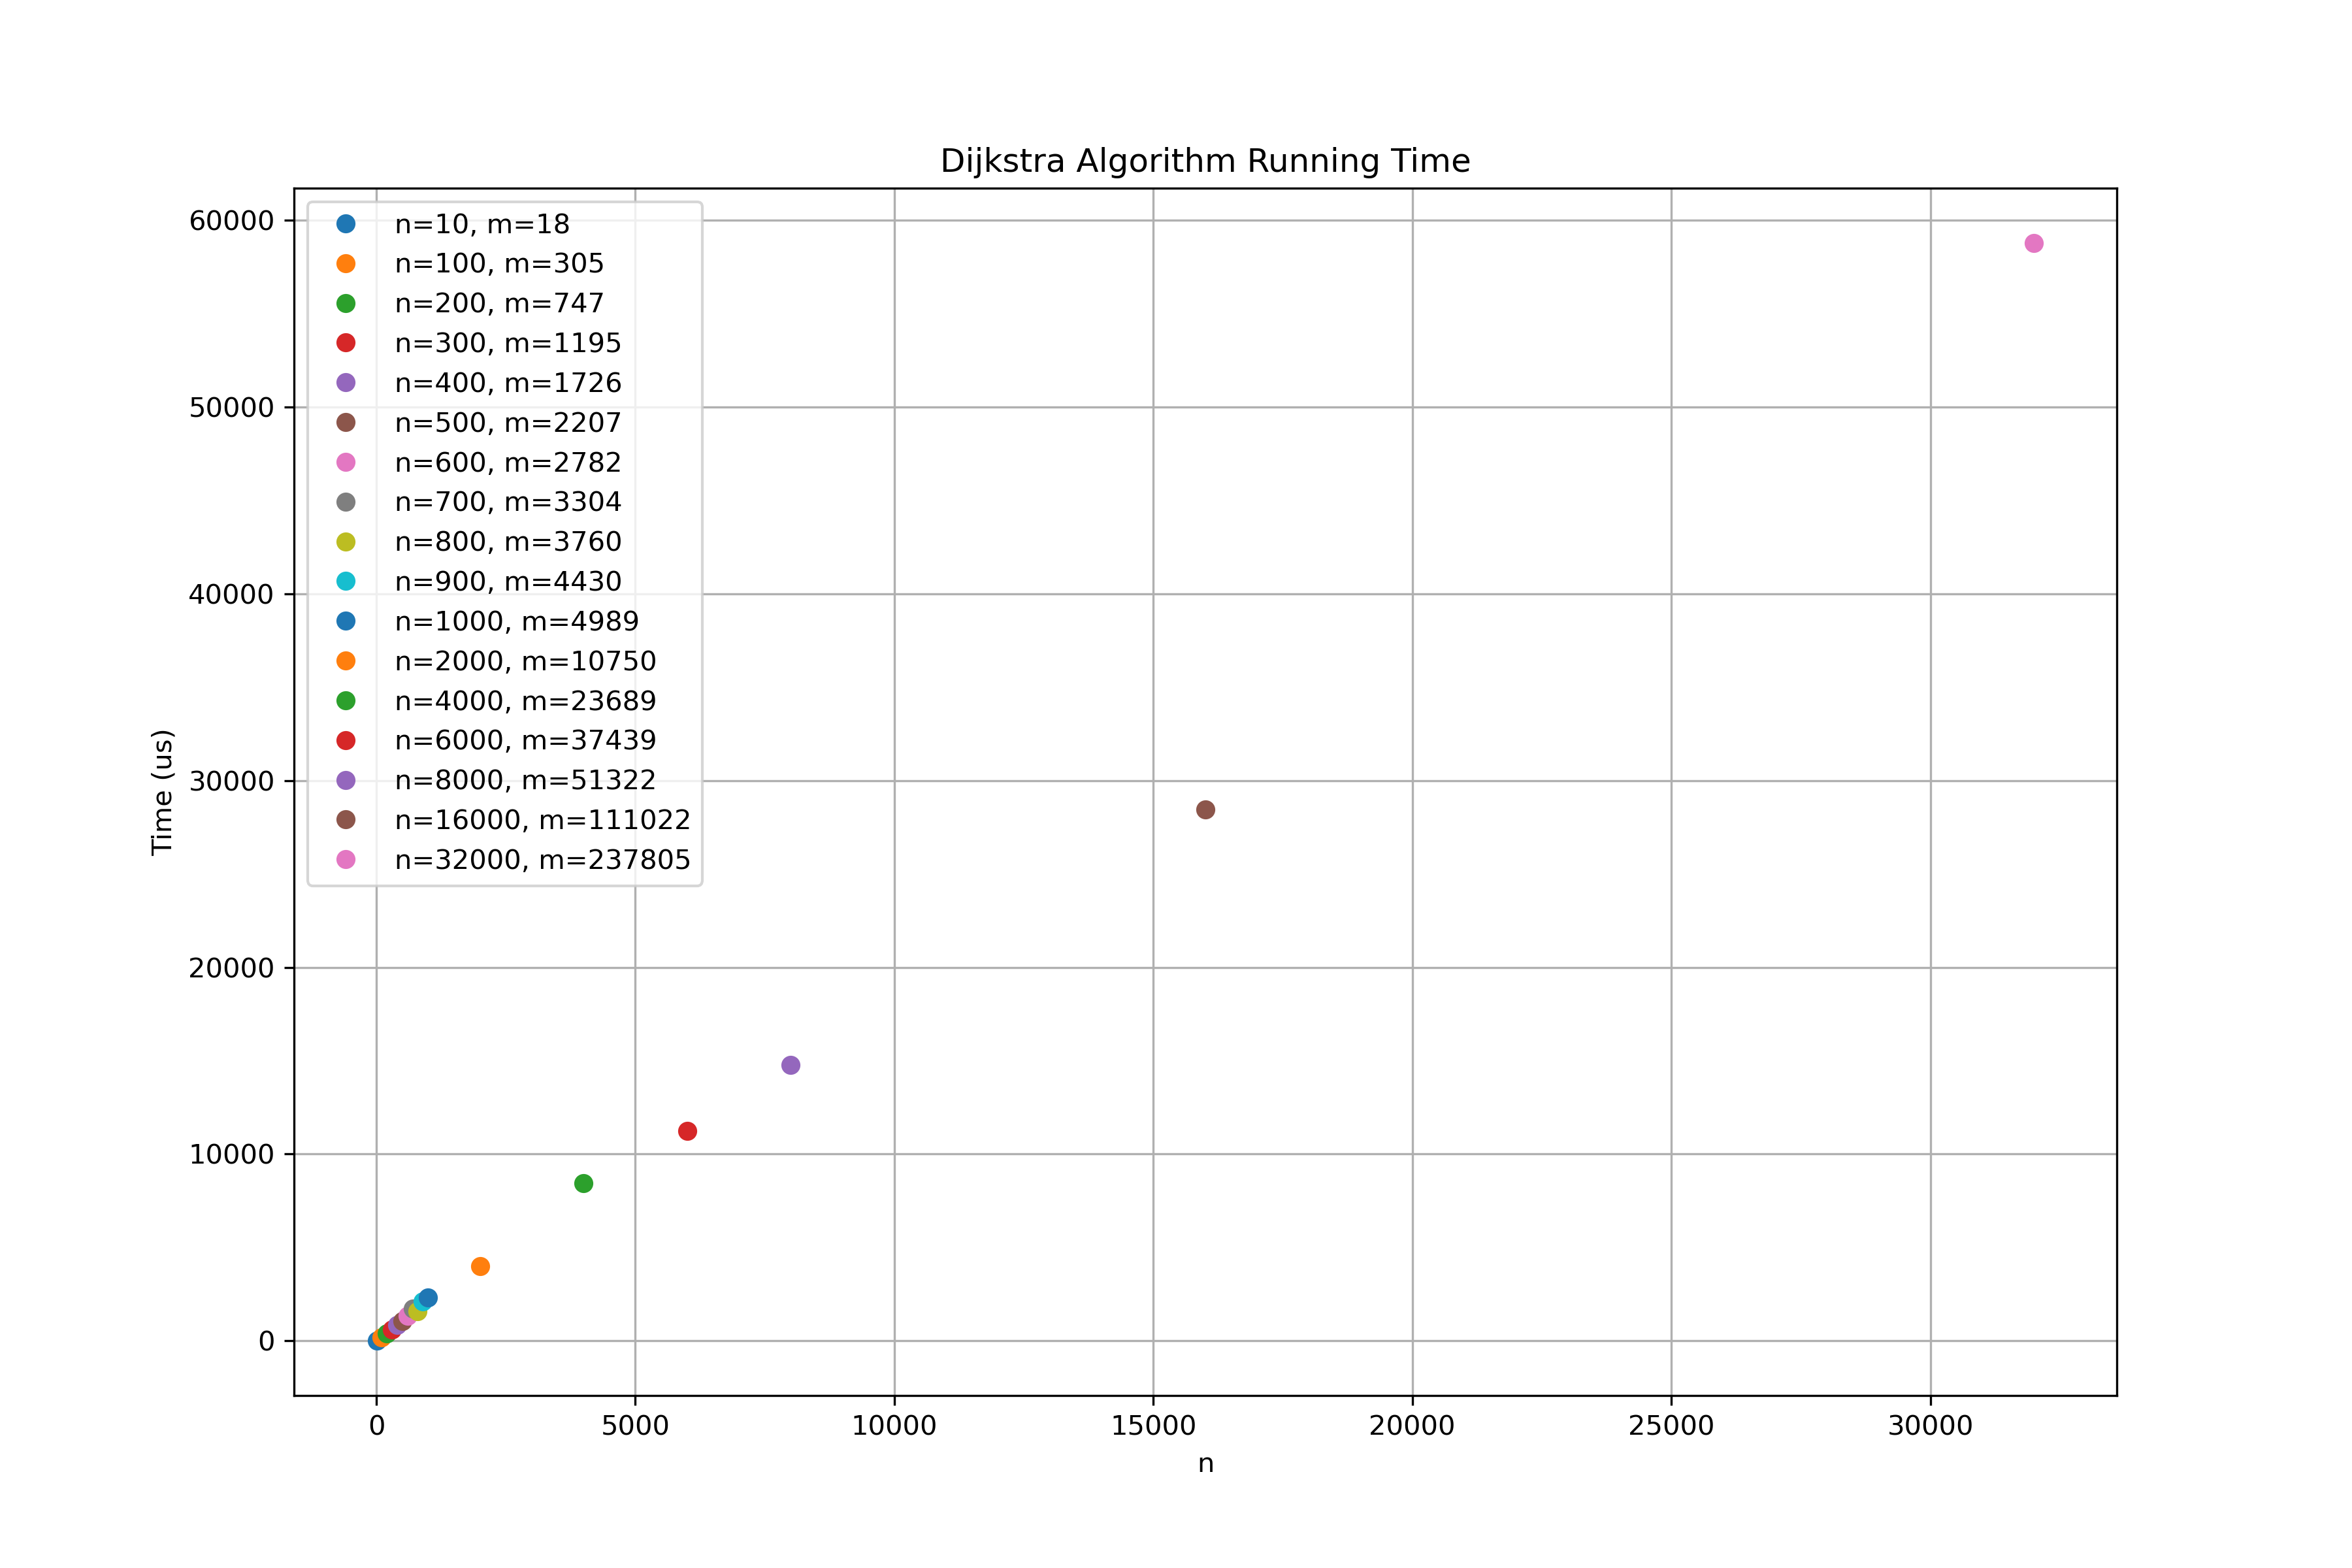
\includegraphics[width=\textwidth]{../results/Dijkstra_running_time.png}
      \caption{Dijkstra's Algorithm}
  \end{subfigure}
  \hfill
  \begin{subfigure}[b]{0.45\textwidth}
      \centering
      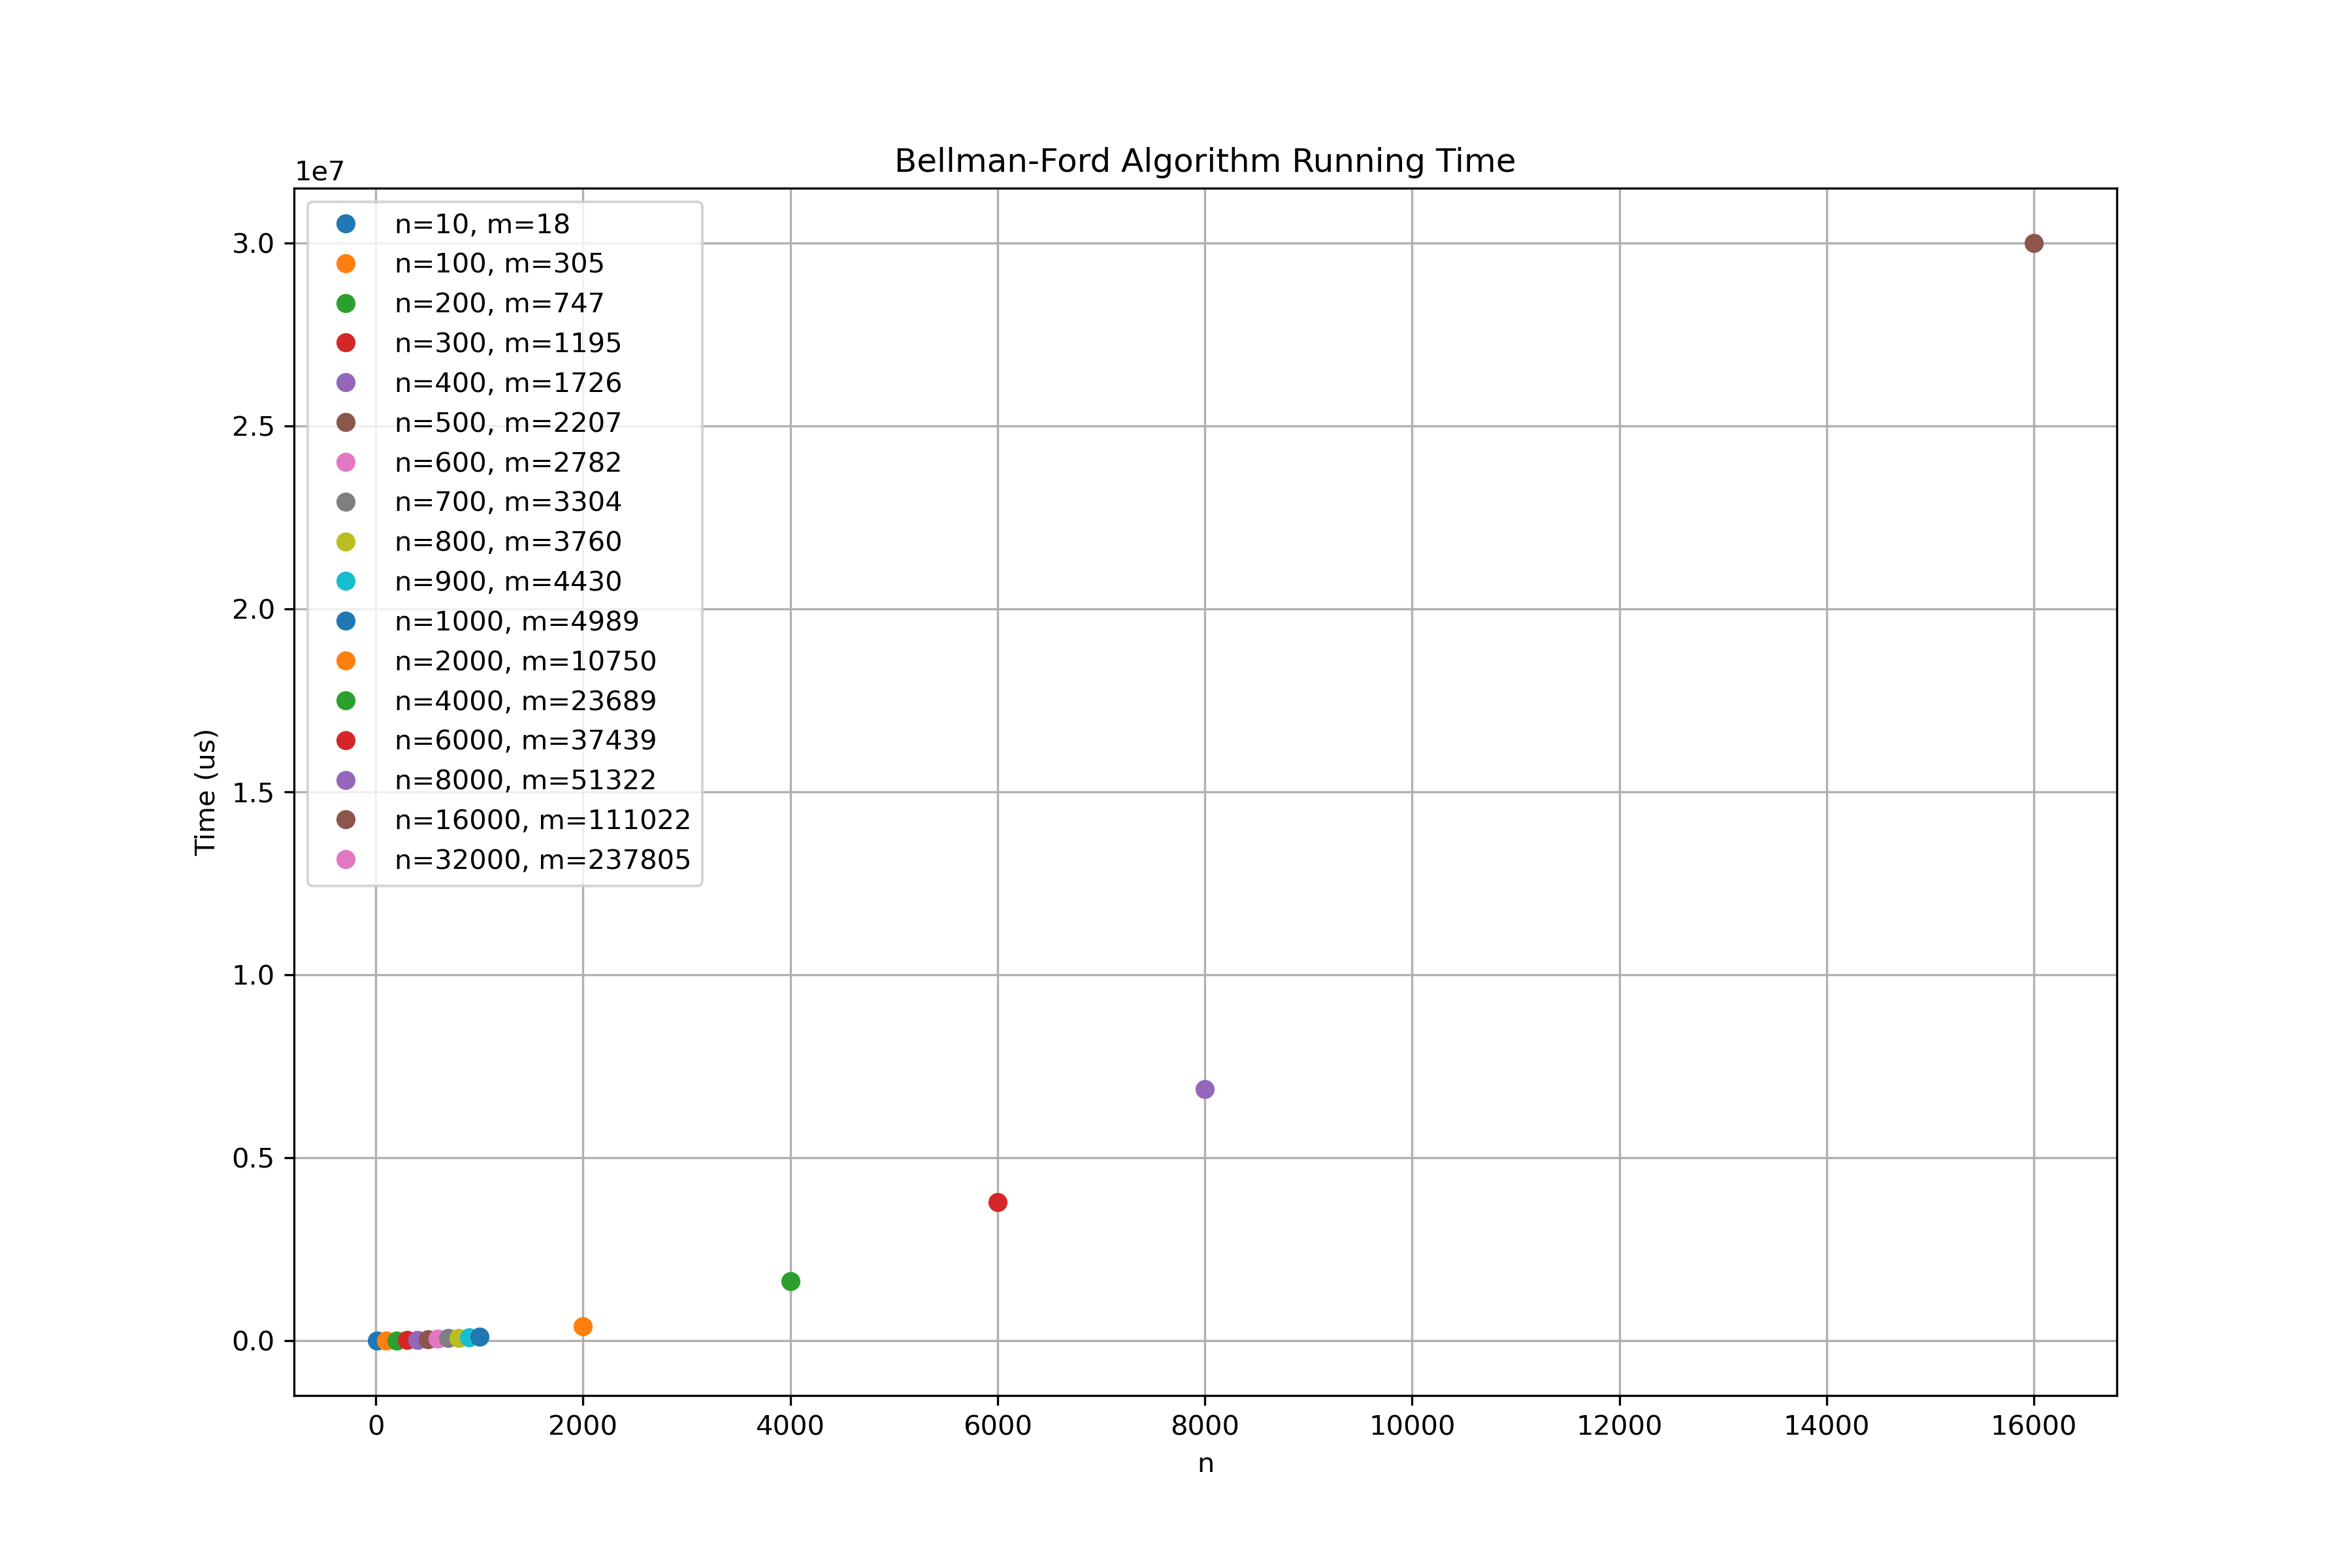
\includegraphics[width=\textwidth]{../results/Bellman-Ford_running_time.png}
      \caption{Bellman-Ford Algorithm}
  \end{subfigure}
  \vfill
  \begin{subfigure}[b]{0.45\textwidth}
      \centering
      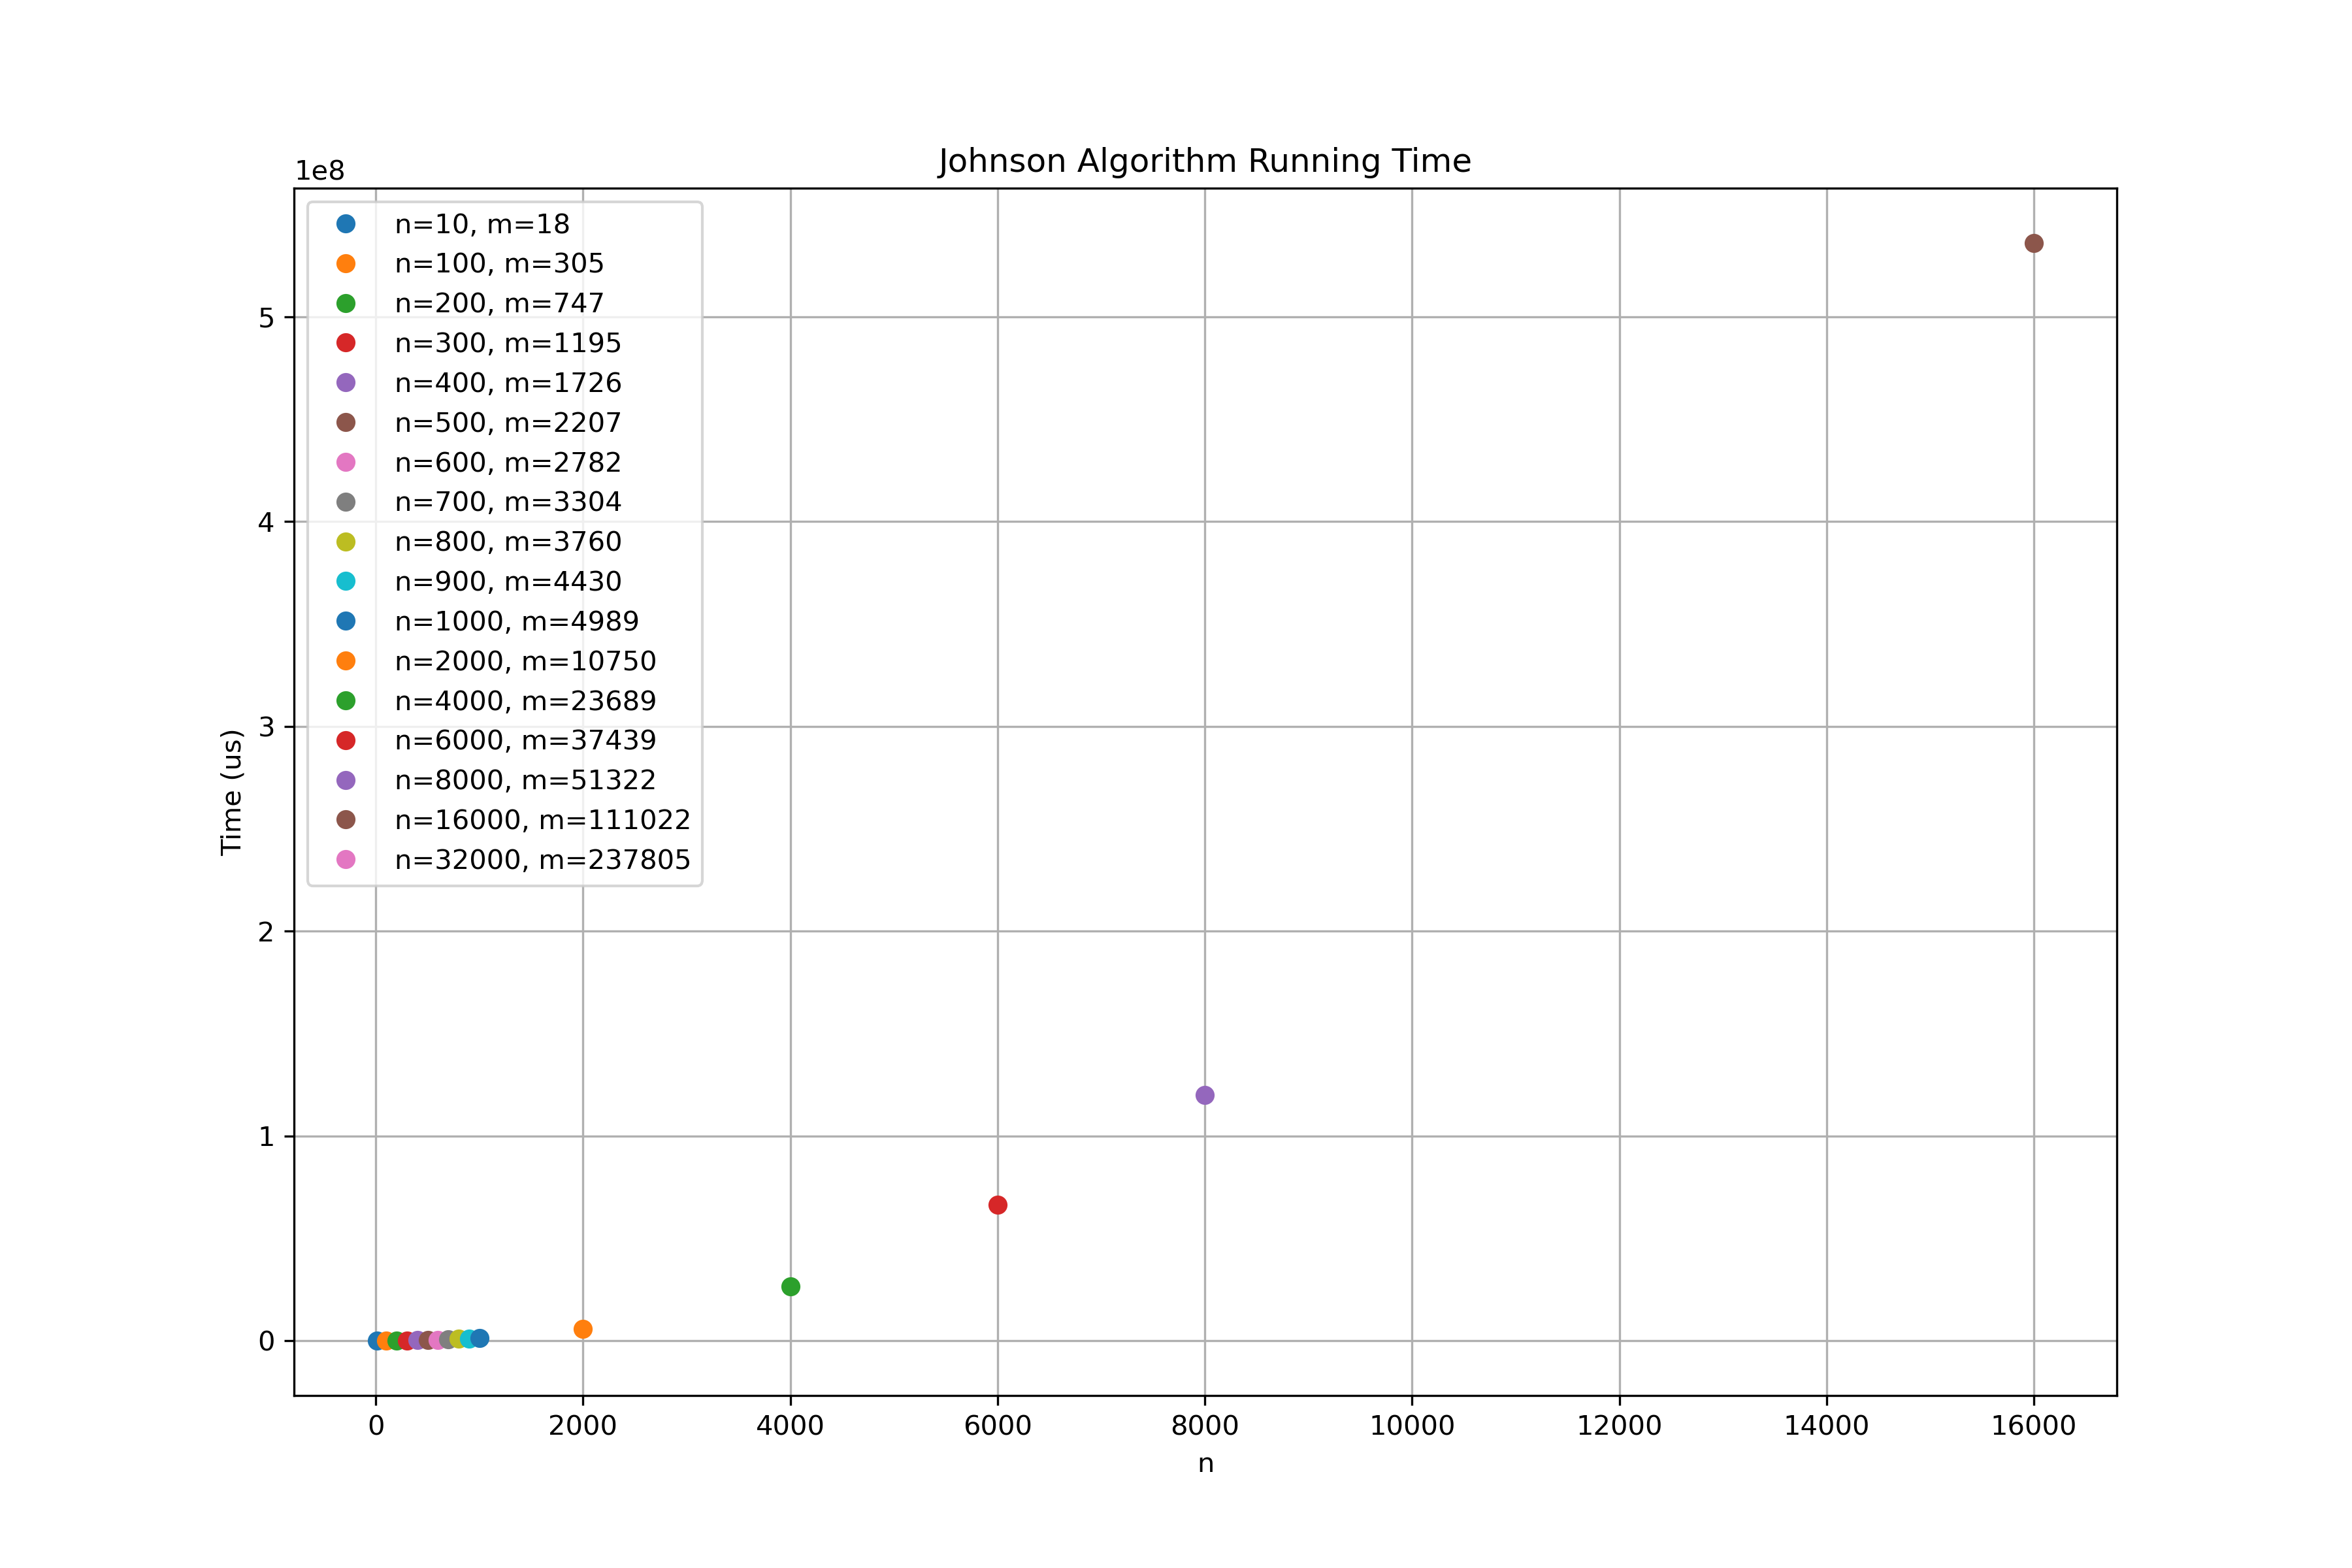
\includegraphics[width=\textwidth]{../results/Johnson_running_time.png}
      \caption{Johnson's Algorithm}
  \end{subfigure}
  \hfill
  \begin{subfigure}[b]{0.45\textwidth}
      \centering
      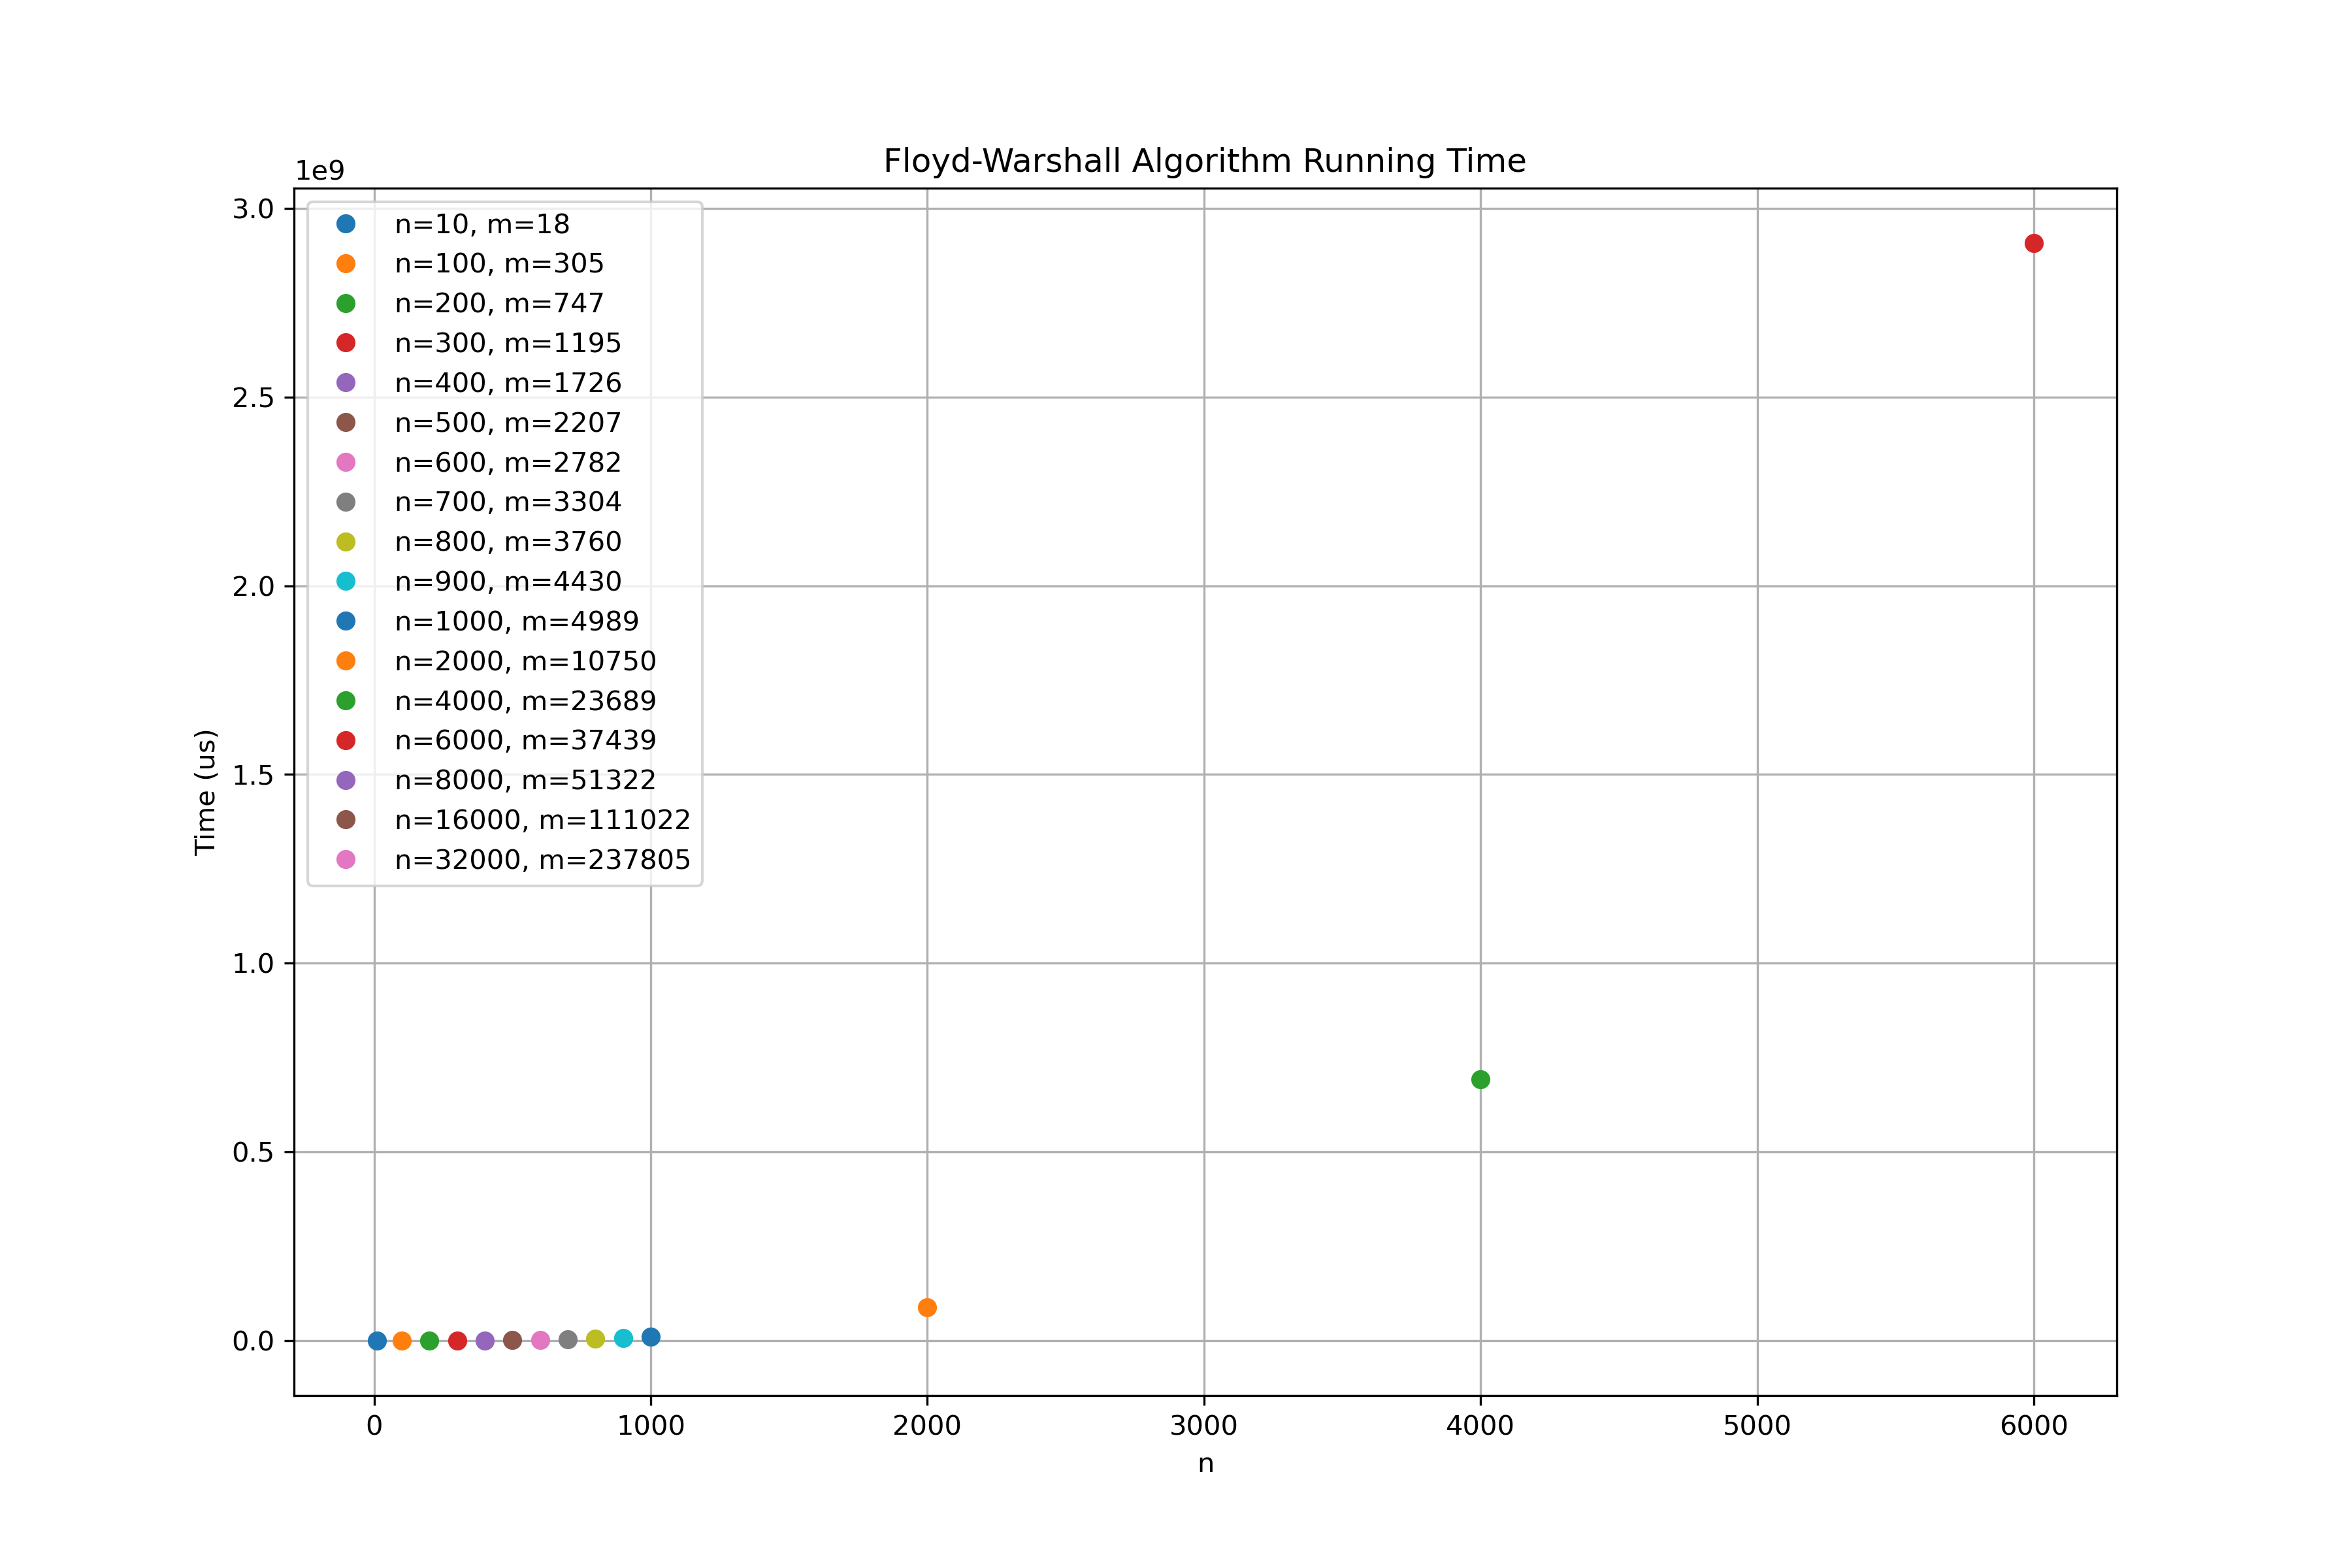
\includegraphics[width=\textwidth]{../results/Floyd-Warshall_running_time.png}
      \caption{Floyd-Warshall Algorithm}
  \end{subfigure}
  \vfill
  \begin{subfigure}[b]{0.45\textwidth}
      \centering
      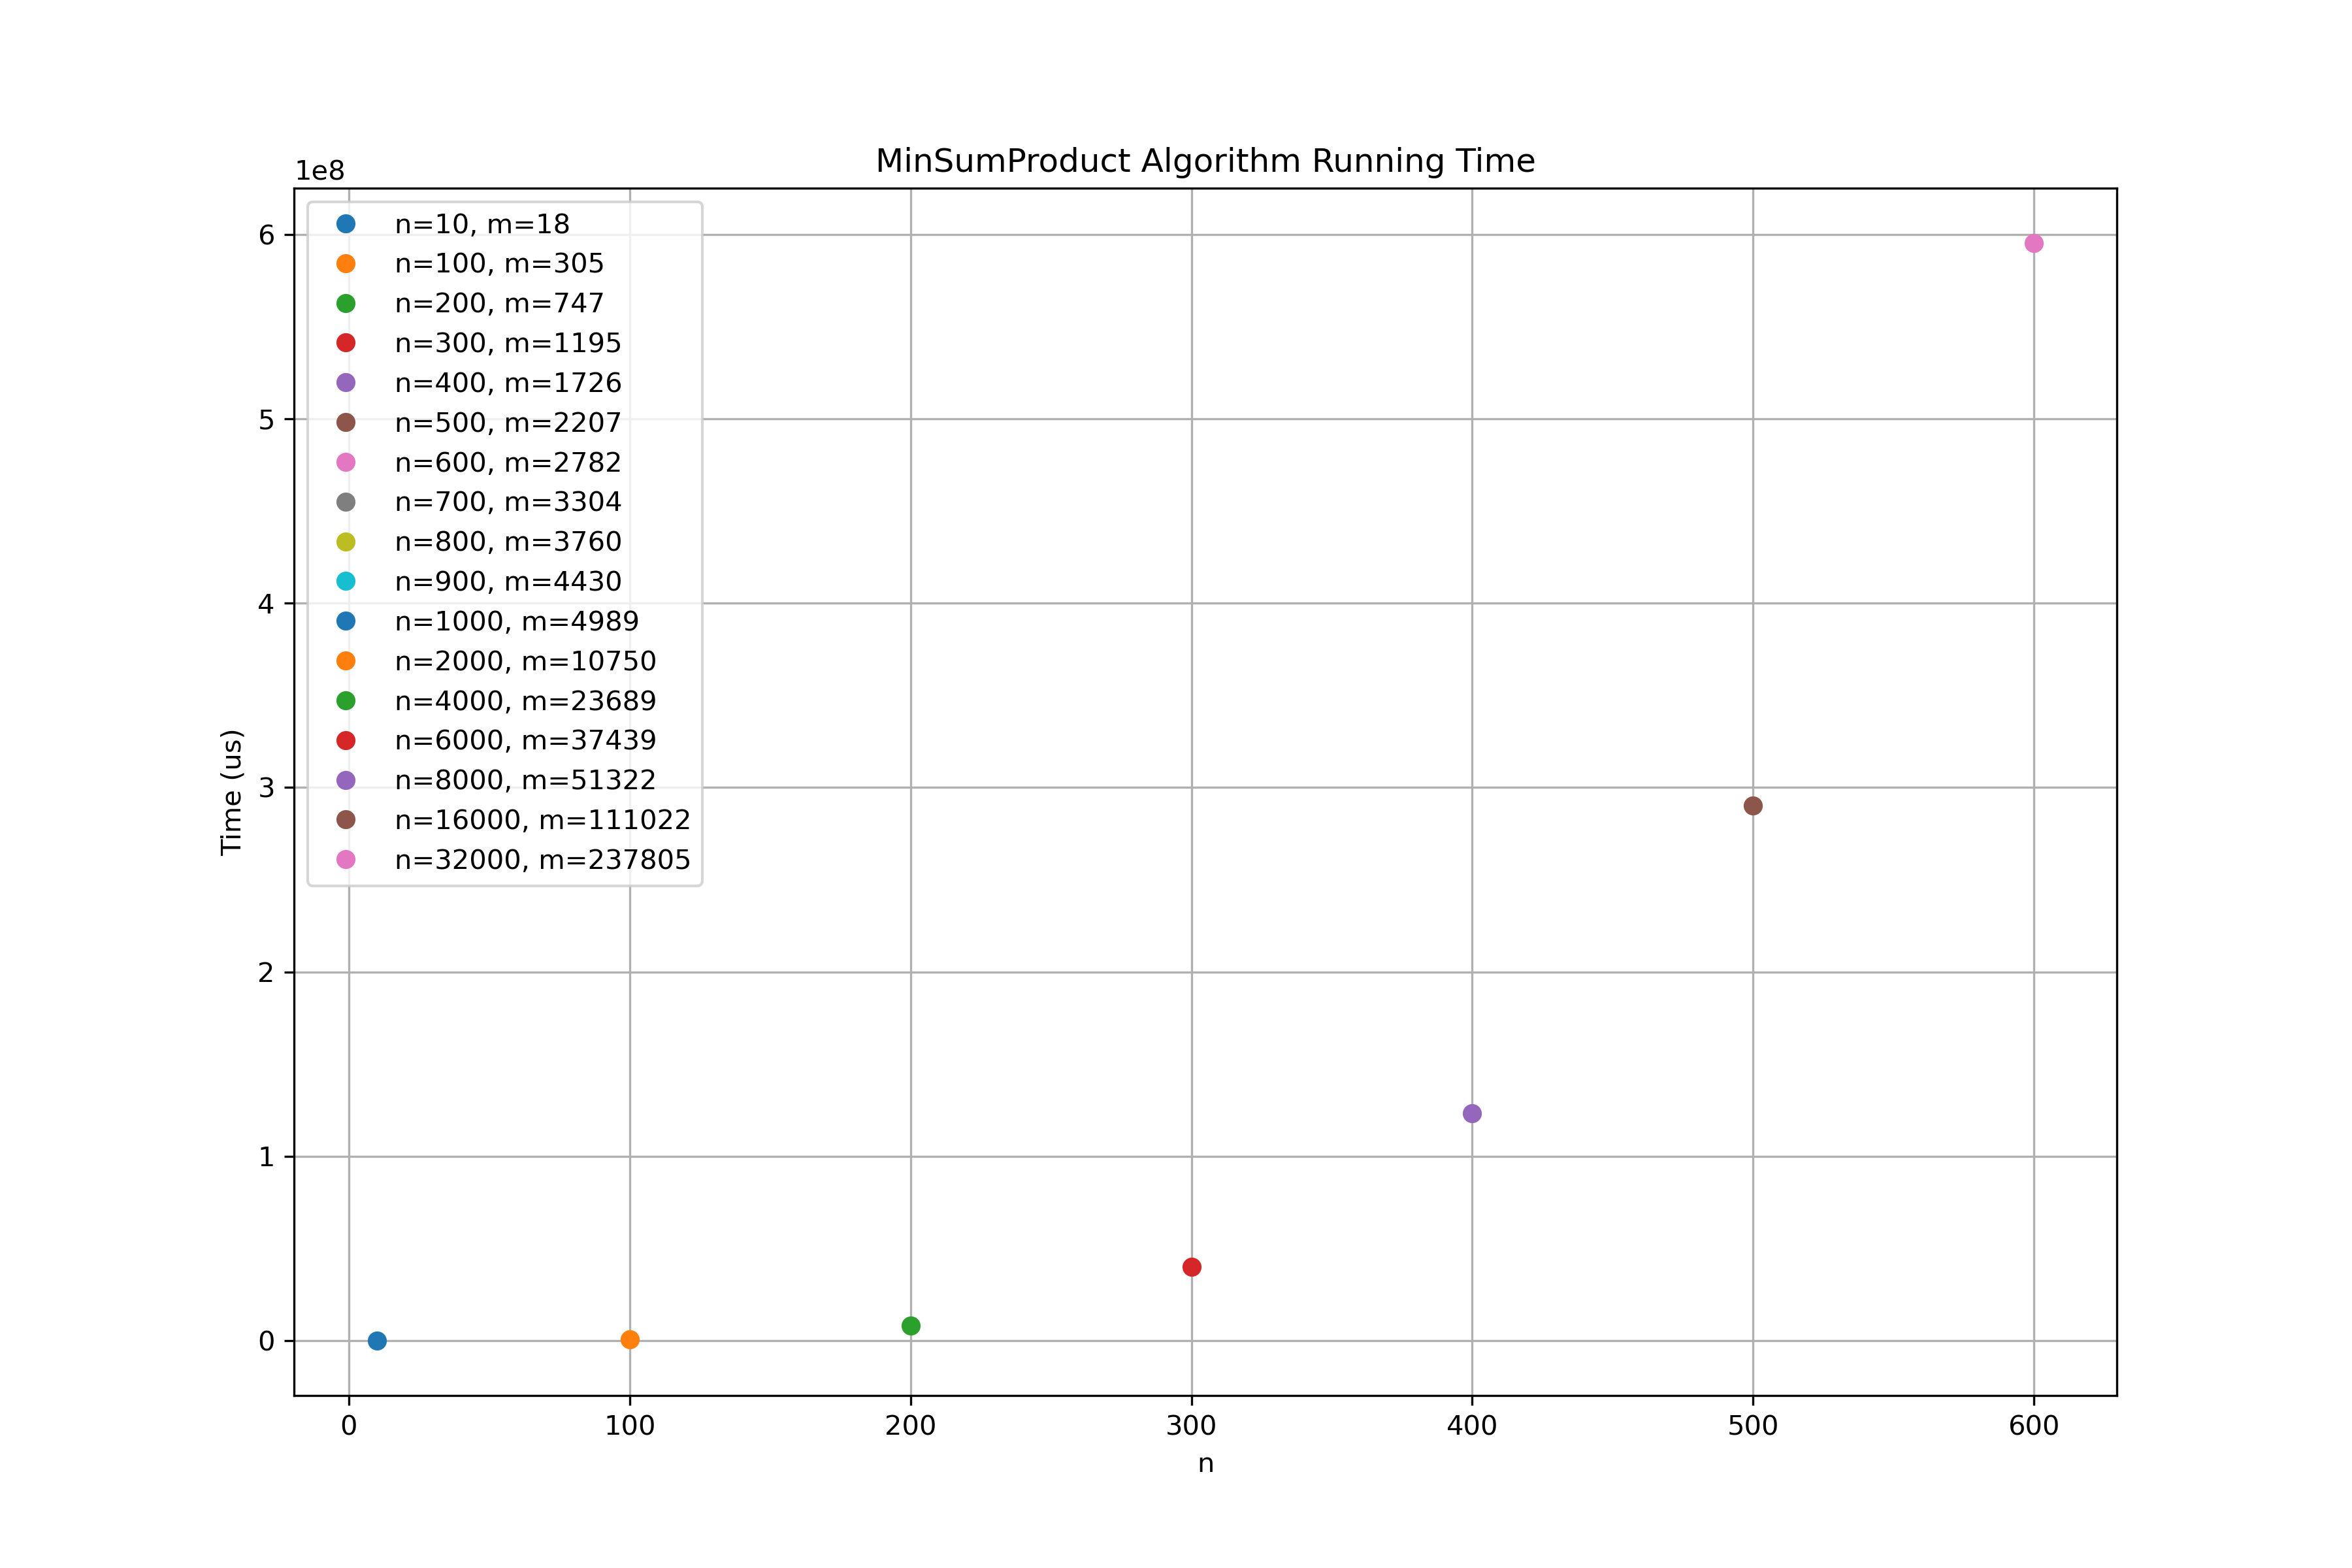
\includegraphics[width=\textwidth]{../results/MinSumProduct_running_time.png}
      \caption{Min-Sum Products}
  \end{subfigure}
  \caption{Different Algorithm runtime - number of nodes relationship}
\end{figure}

\subsection{Relationship between running time and big O bounding function}\

\begin{figure}[H]
  \centering
  \begin{subfigure}[b]{0.45\textwidth}
      \centering
      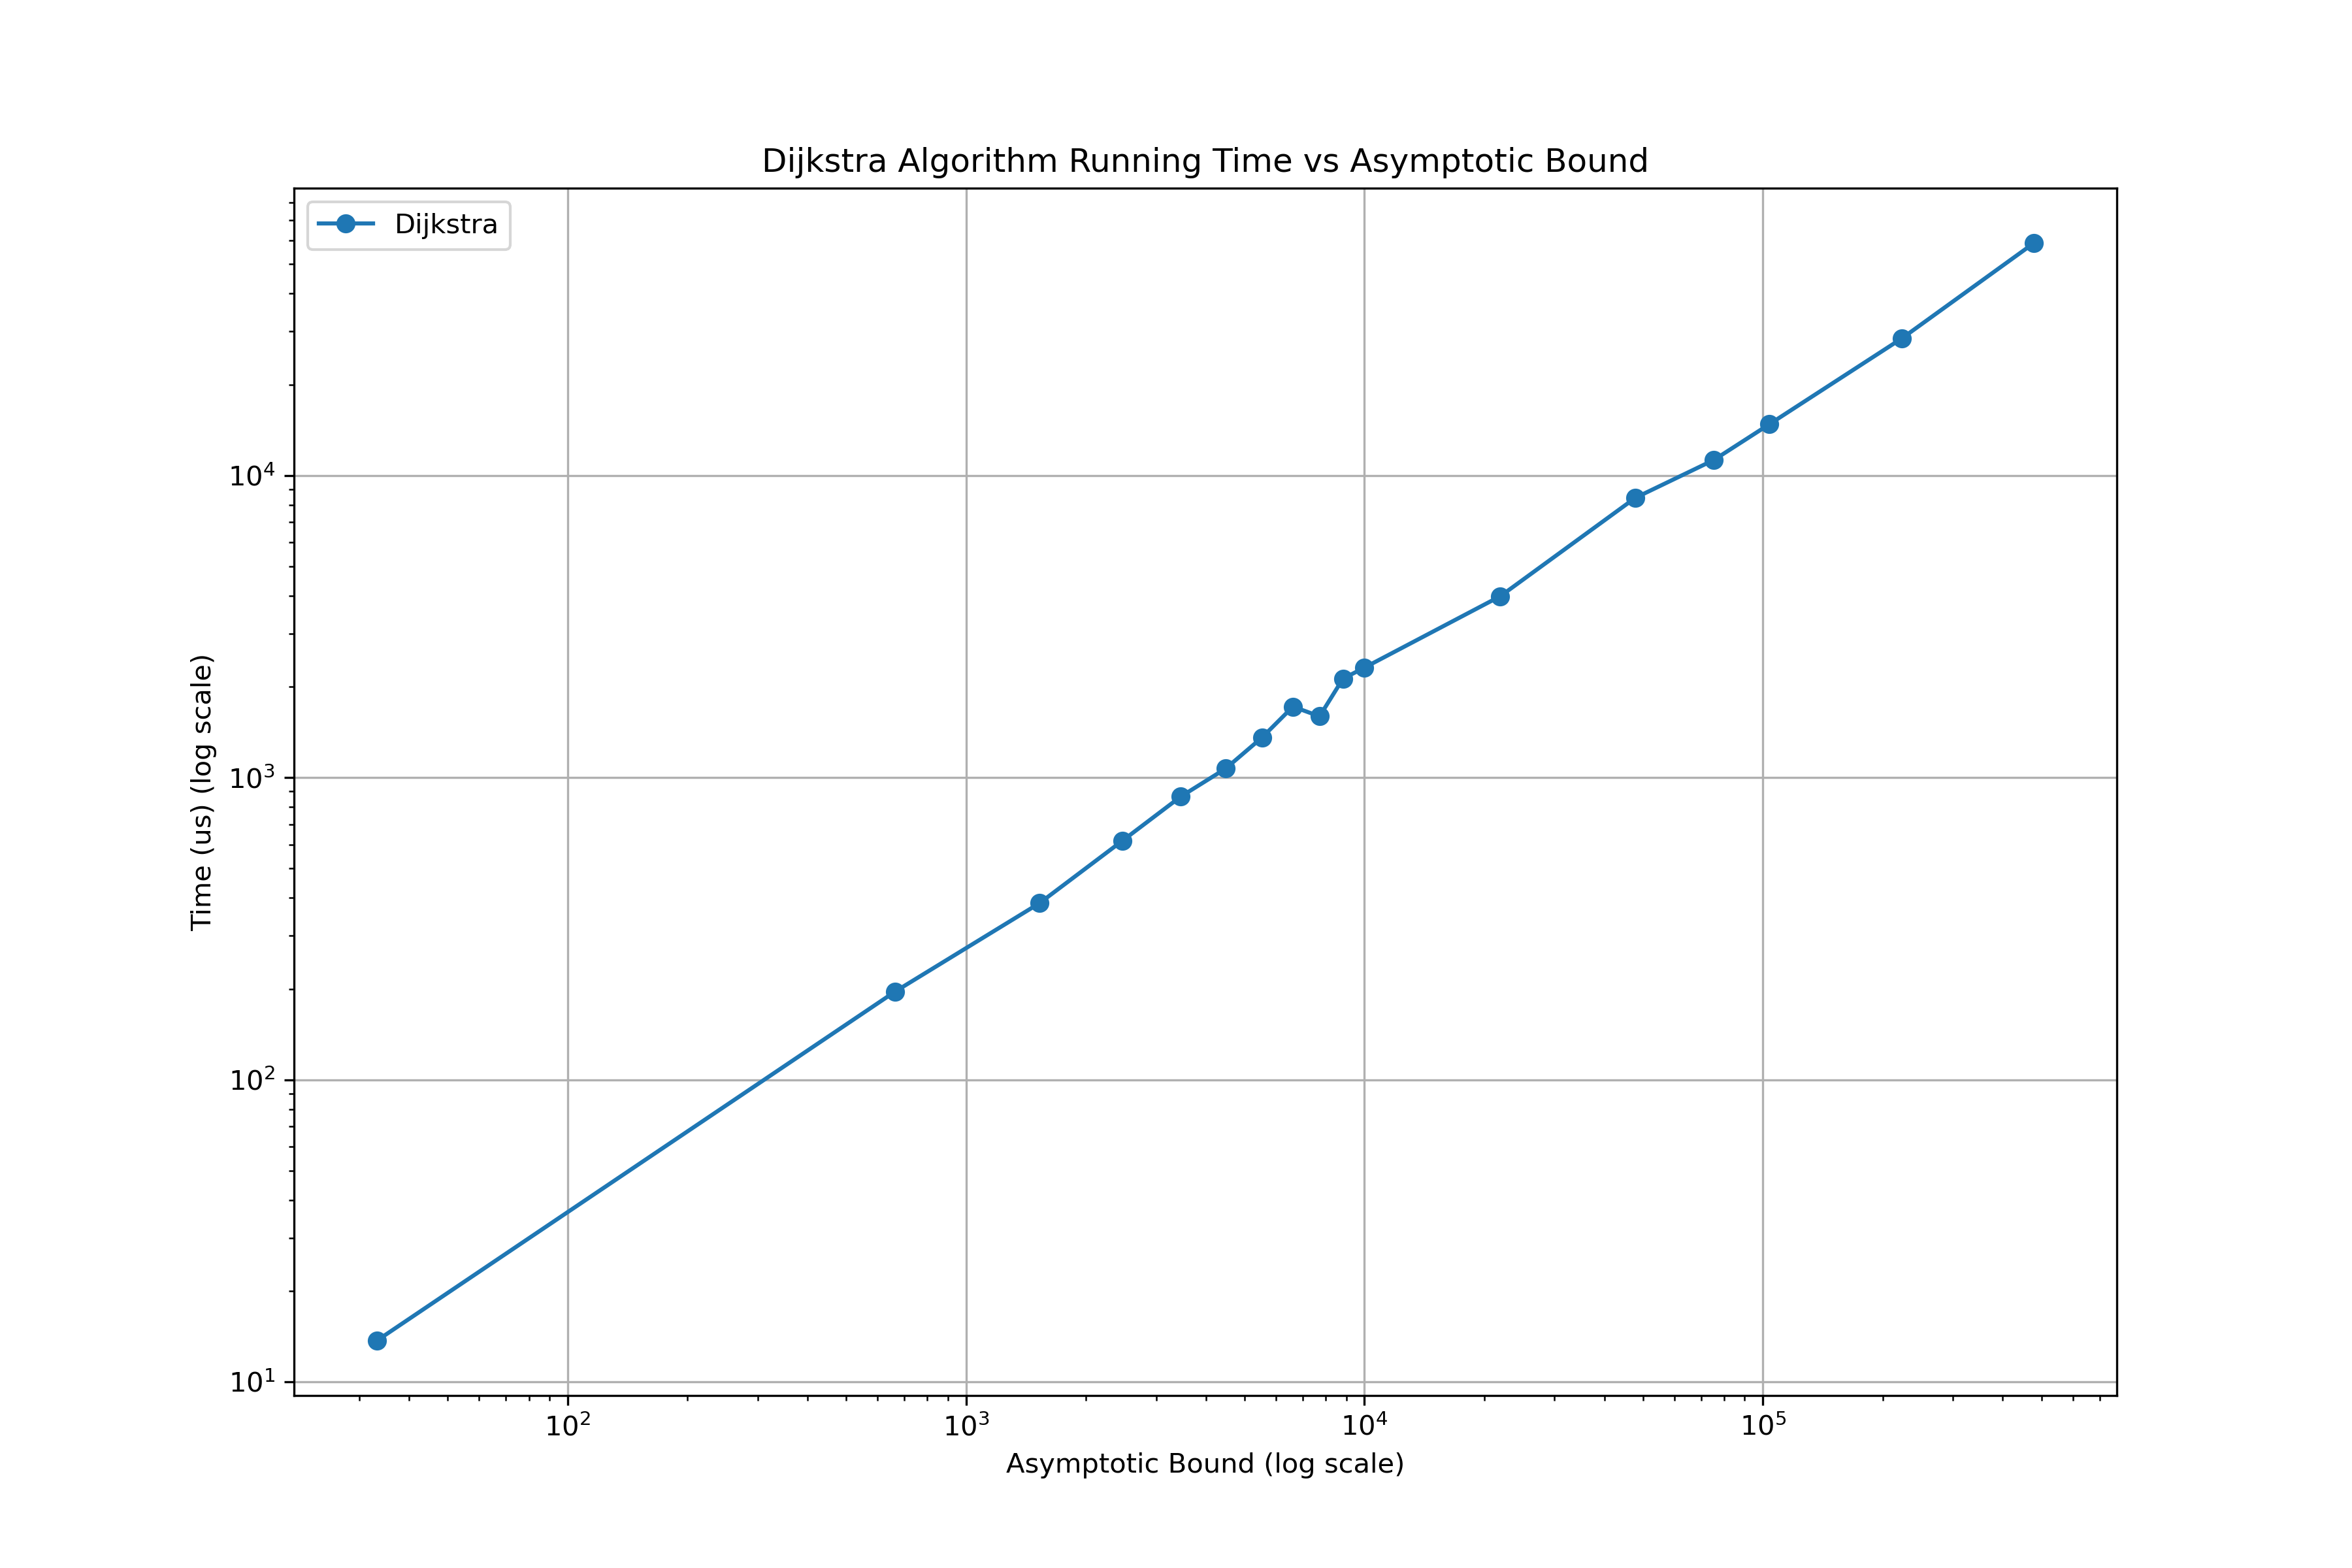
\includegraphics[width=\textwidth]{../results/Dijkstra_running_time_bound.png}
      \caption{Dijkstra's Algorithm}
  \end{subfigure}
  \hfill
  \begin{subfigure}[b]{0.45\textwidth}
      \centering
      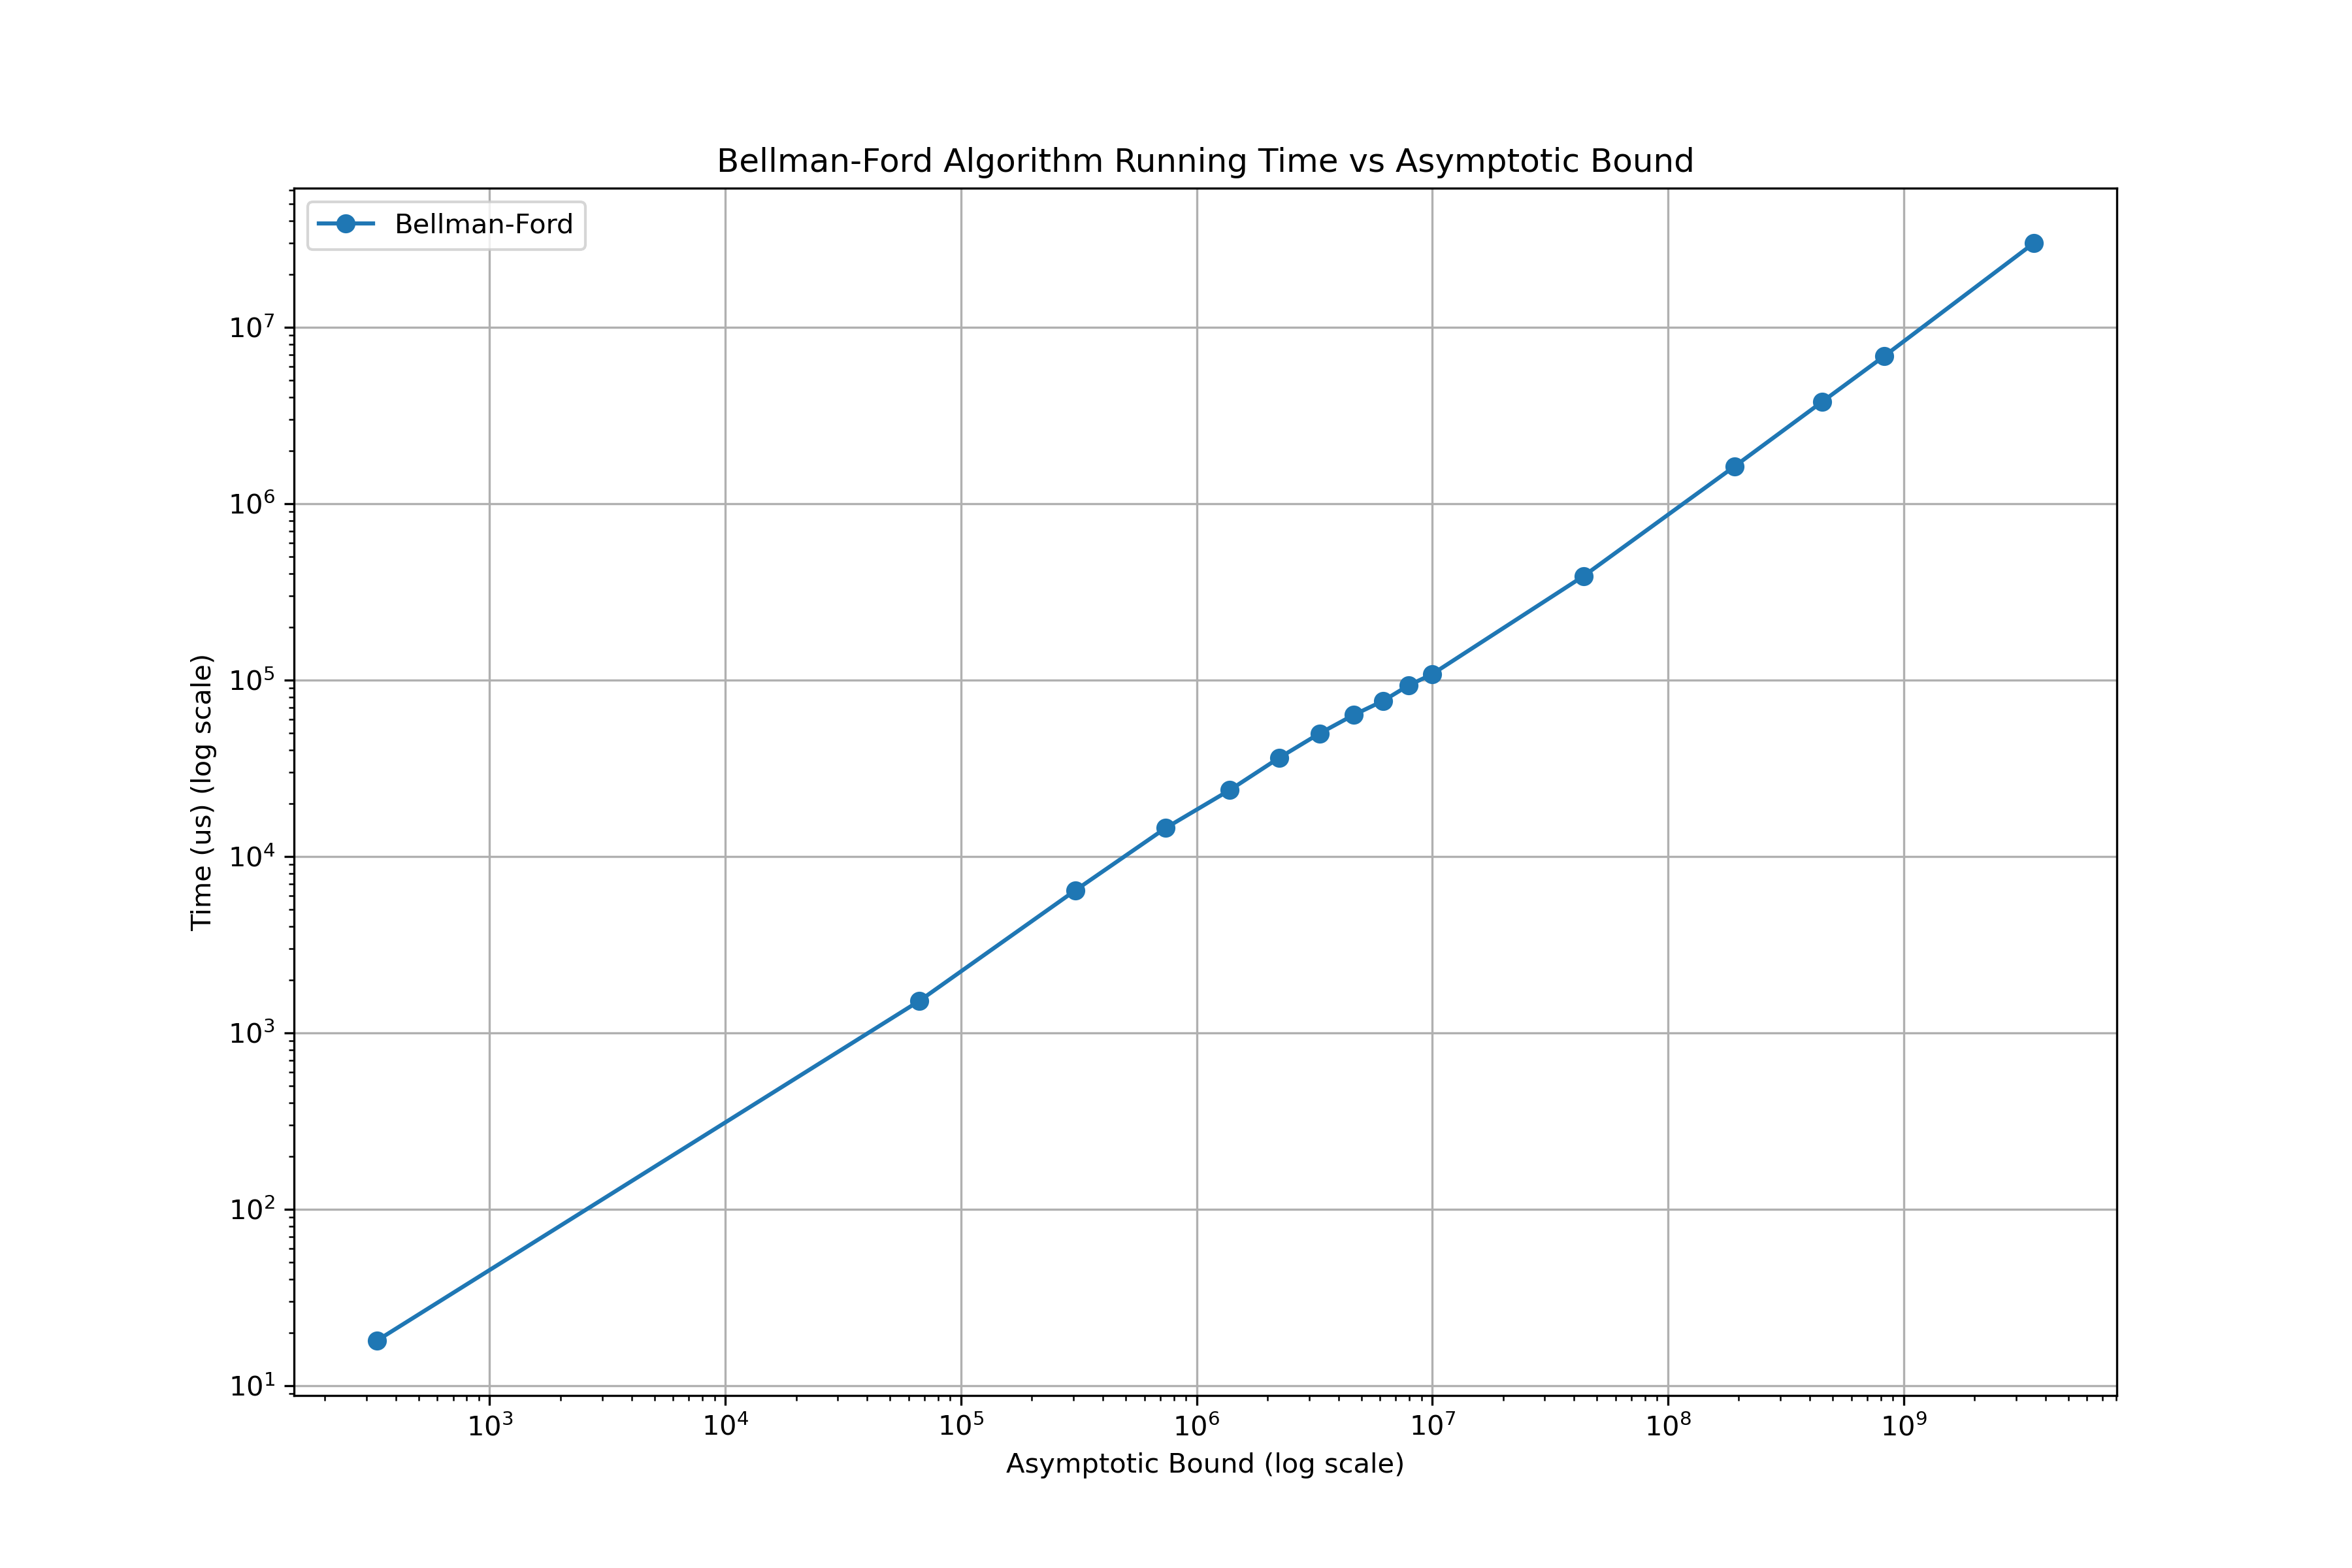
\includegraphics[width=\textwidth]{../results/Bellman-Ford_running_time_bound.png}
      \caption{Bellman-Ford Algorithm}
  \end{subfigure}
  \vfill
  \begin{subfigure}[b]{0.45\textwidth}
      \centering
      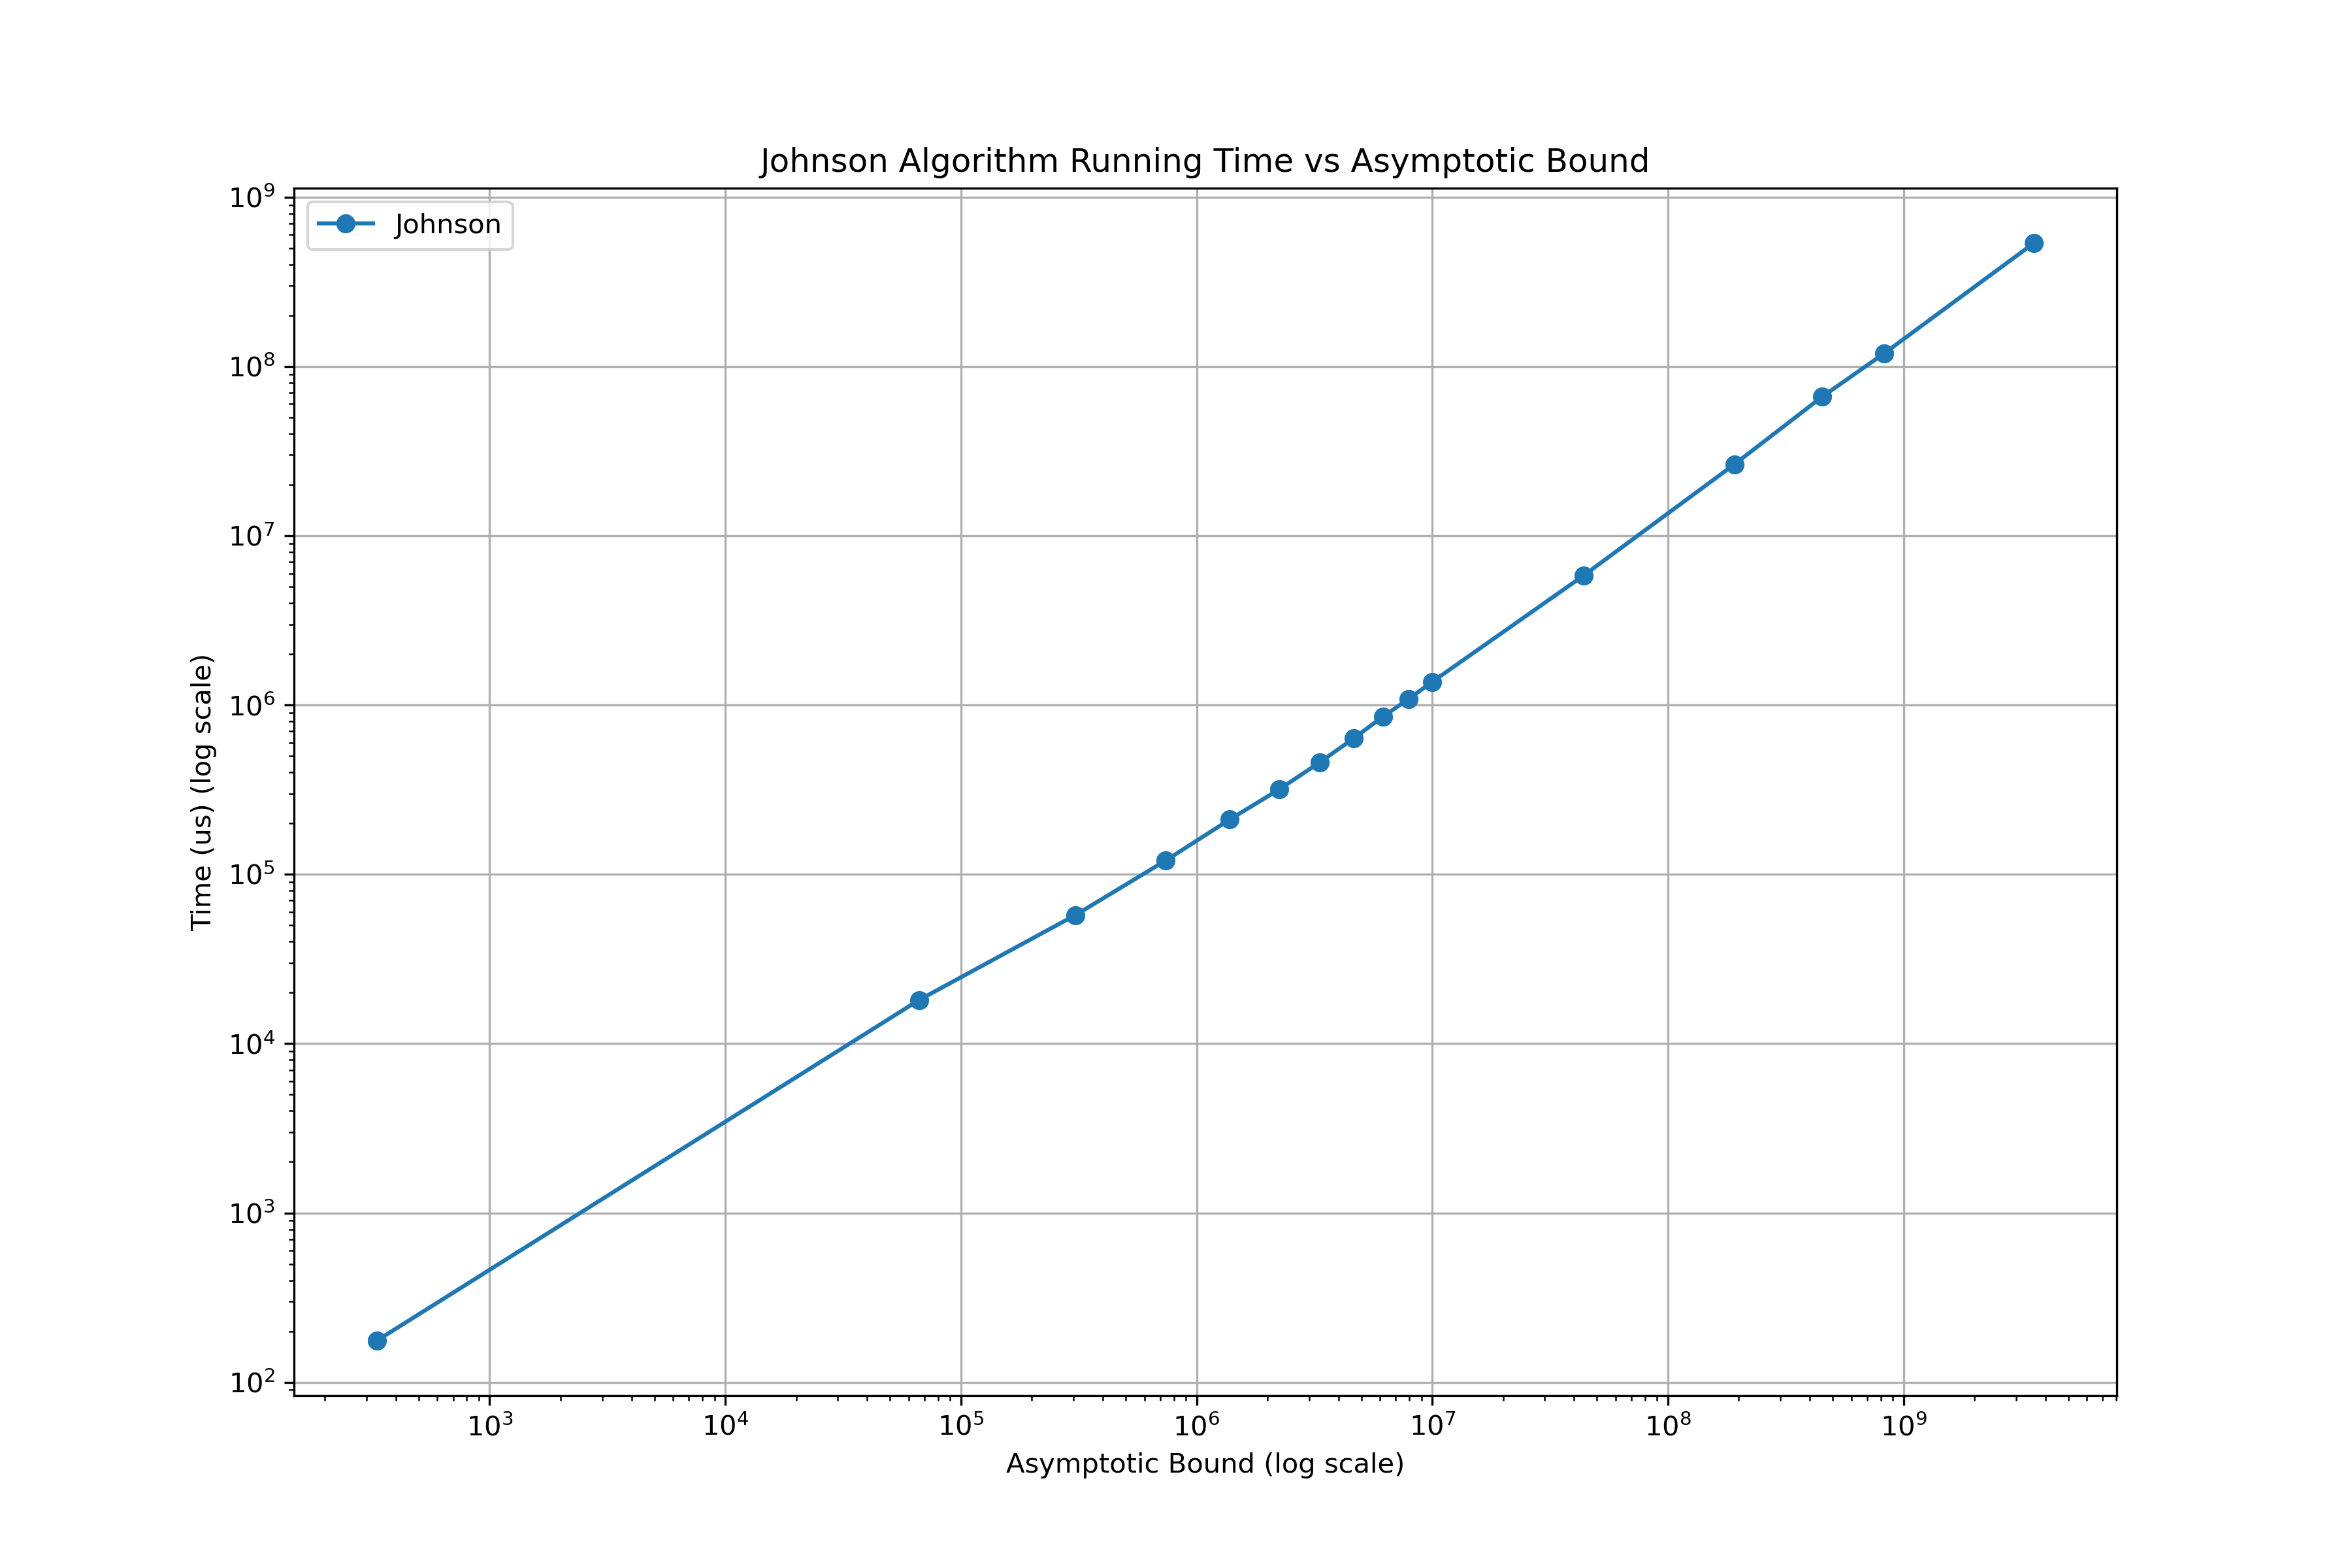
\includegraphics[width=\textwidth]{../results/Johnson_running_time_bound.png}
      \caption{Johnson's Algorithm}
  \end{subfigure}
  \hfill
  \begin{subfigure}[b]{0.45\textwidth}
      \centering
      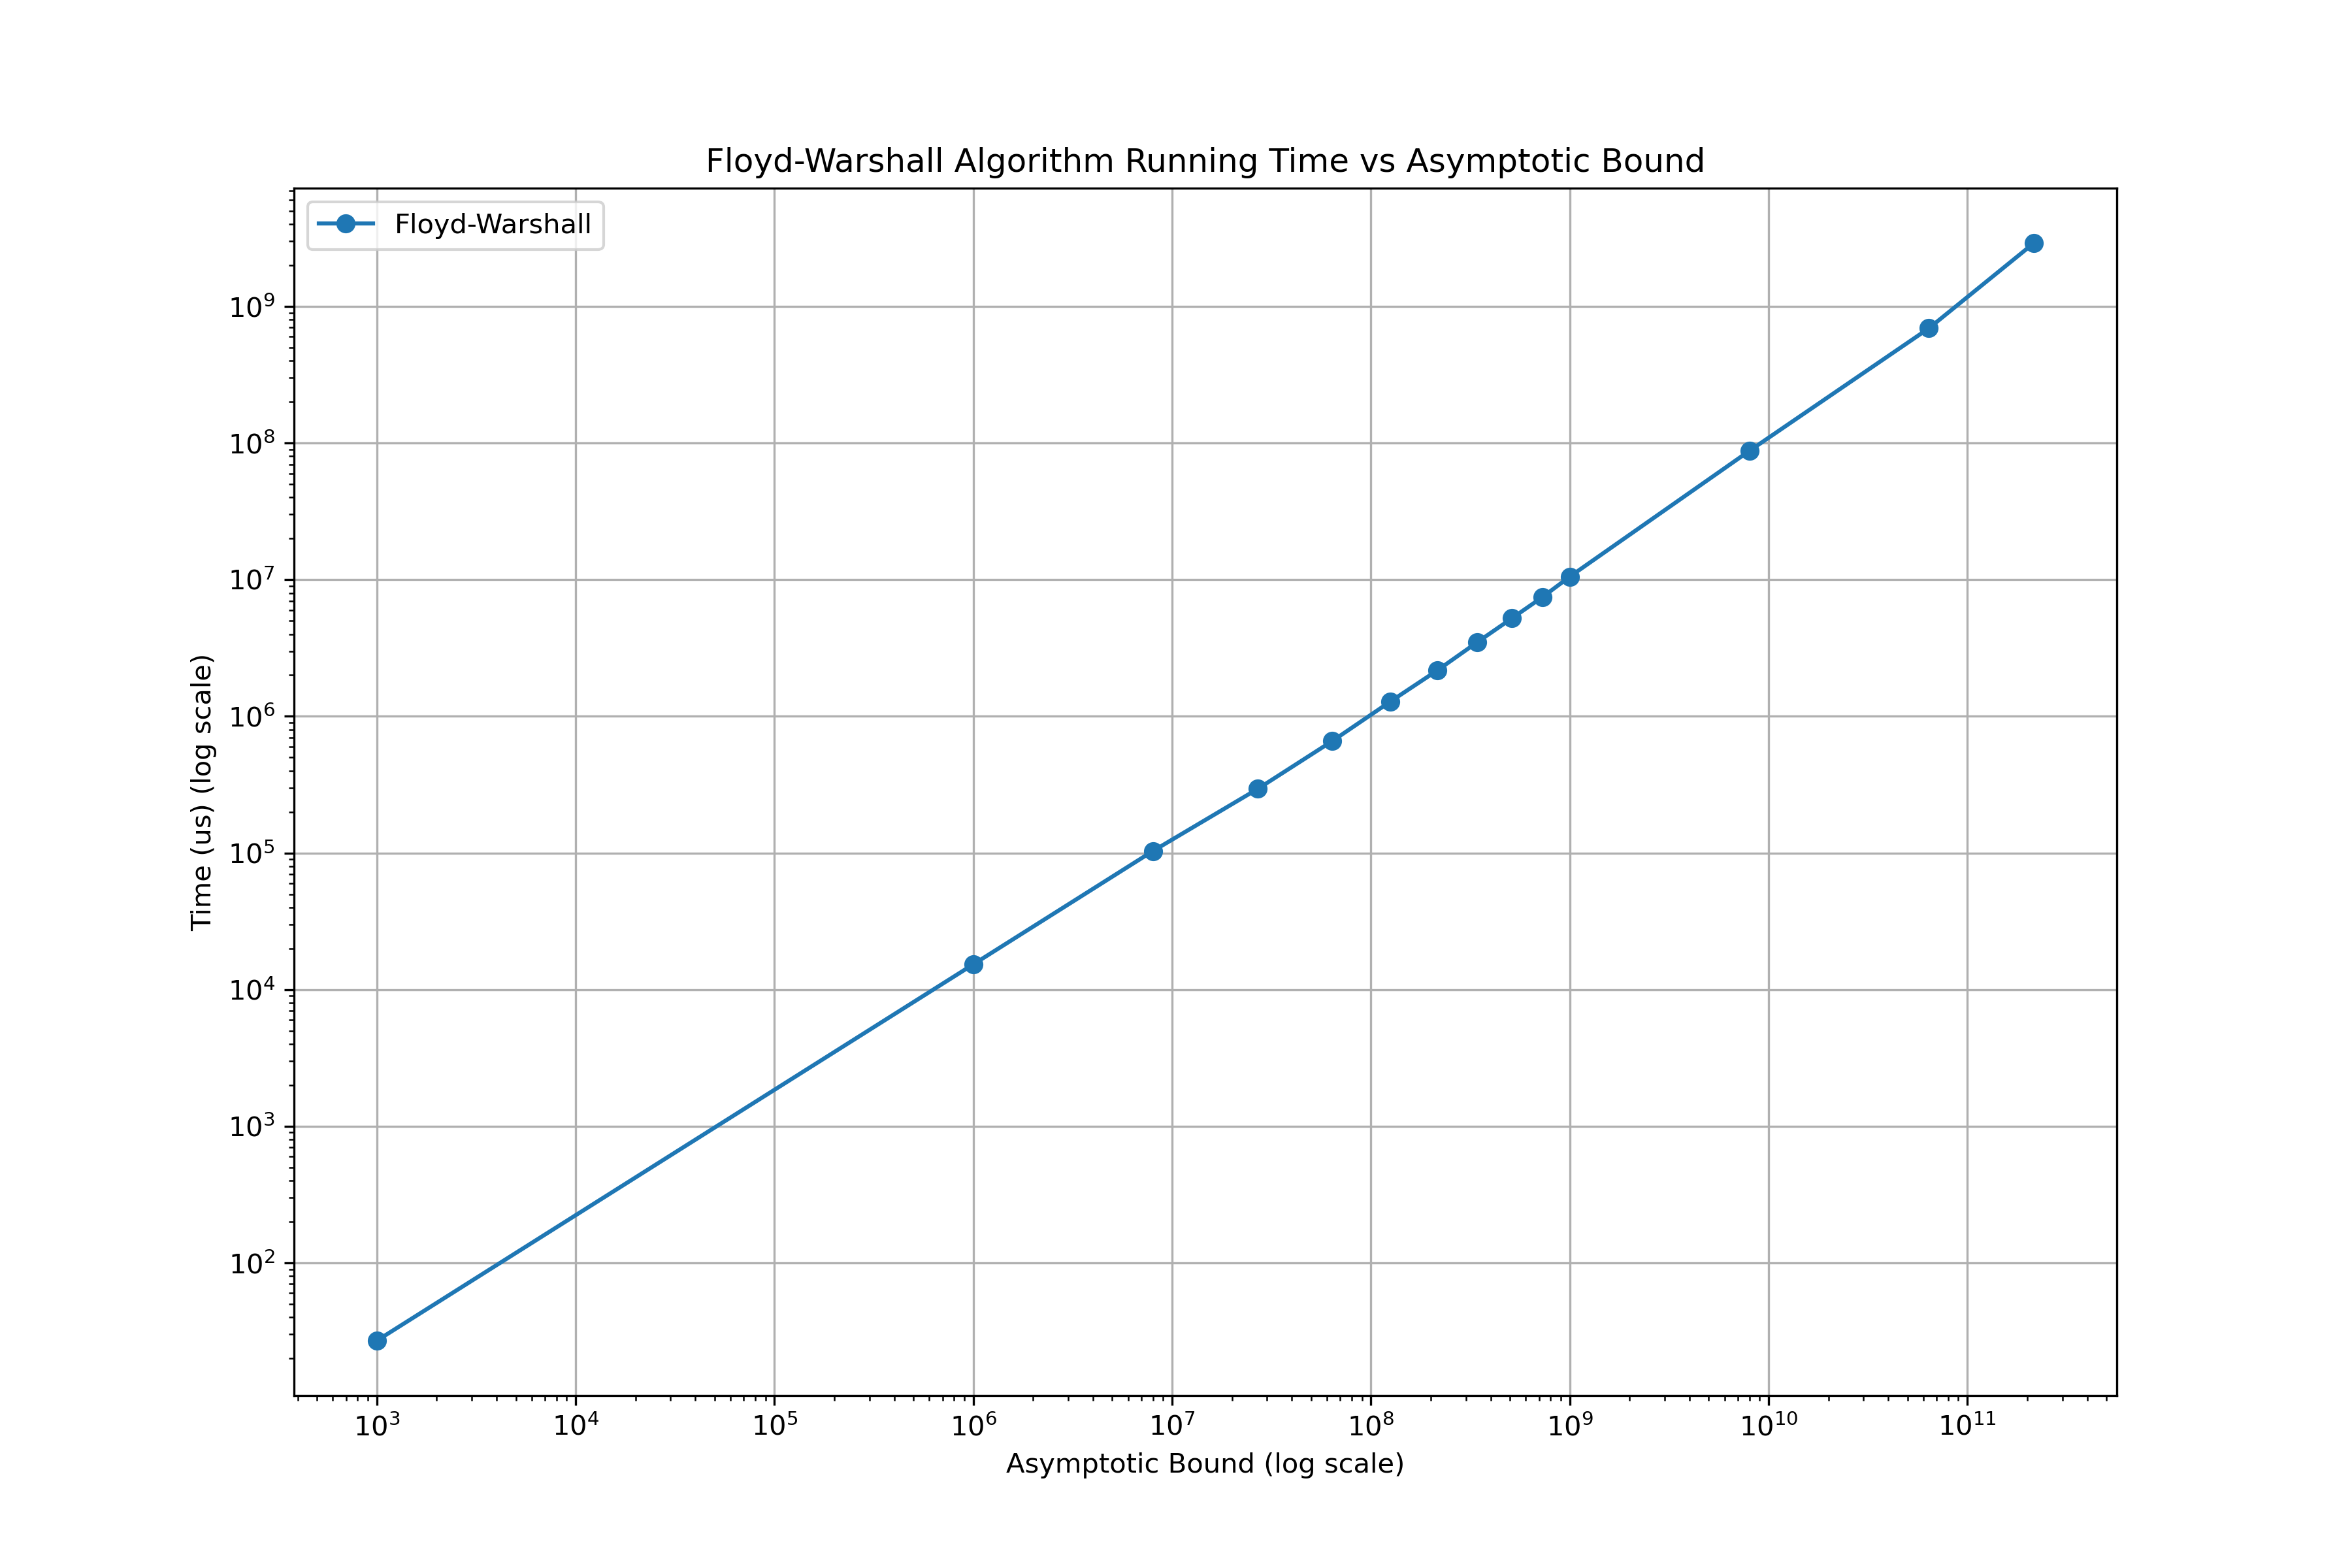
\includegraphics[width=\textwidth]{../results/Floyd-Warshall_running_time_bound.png}
      \caption{Floyd-Warshall Algorithm}
  \end{subfigure}
  \vfill
  \begin{subfigure}[b]{0.45\textwidth}
      \centering
      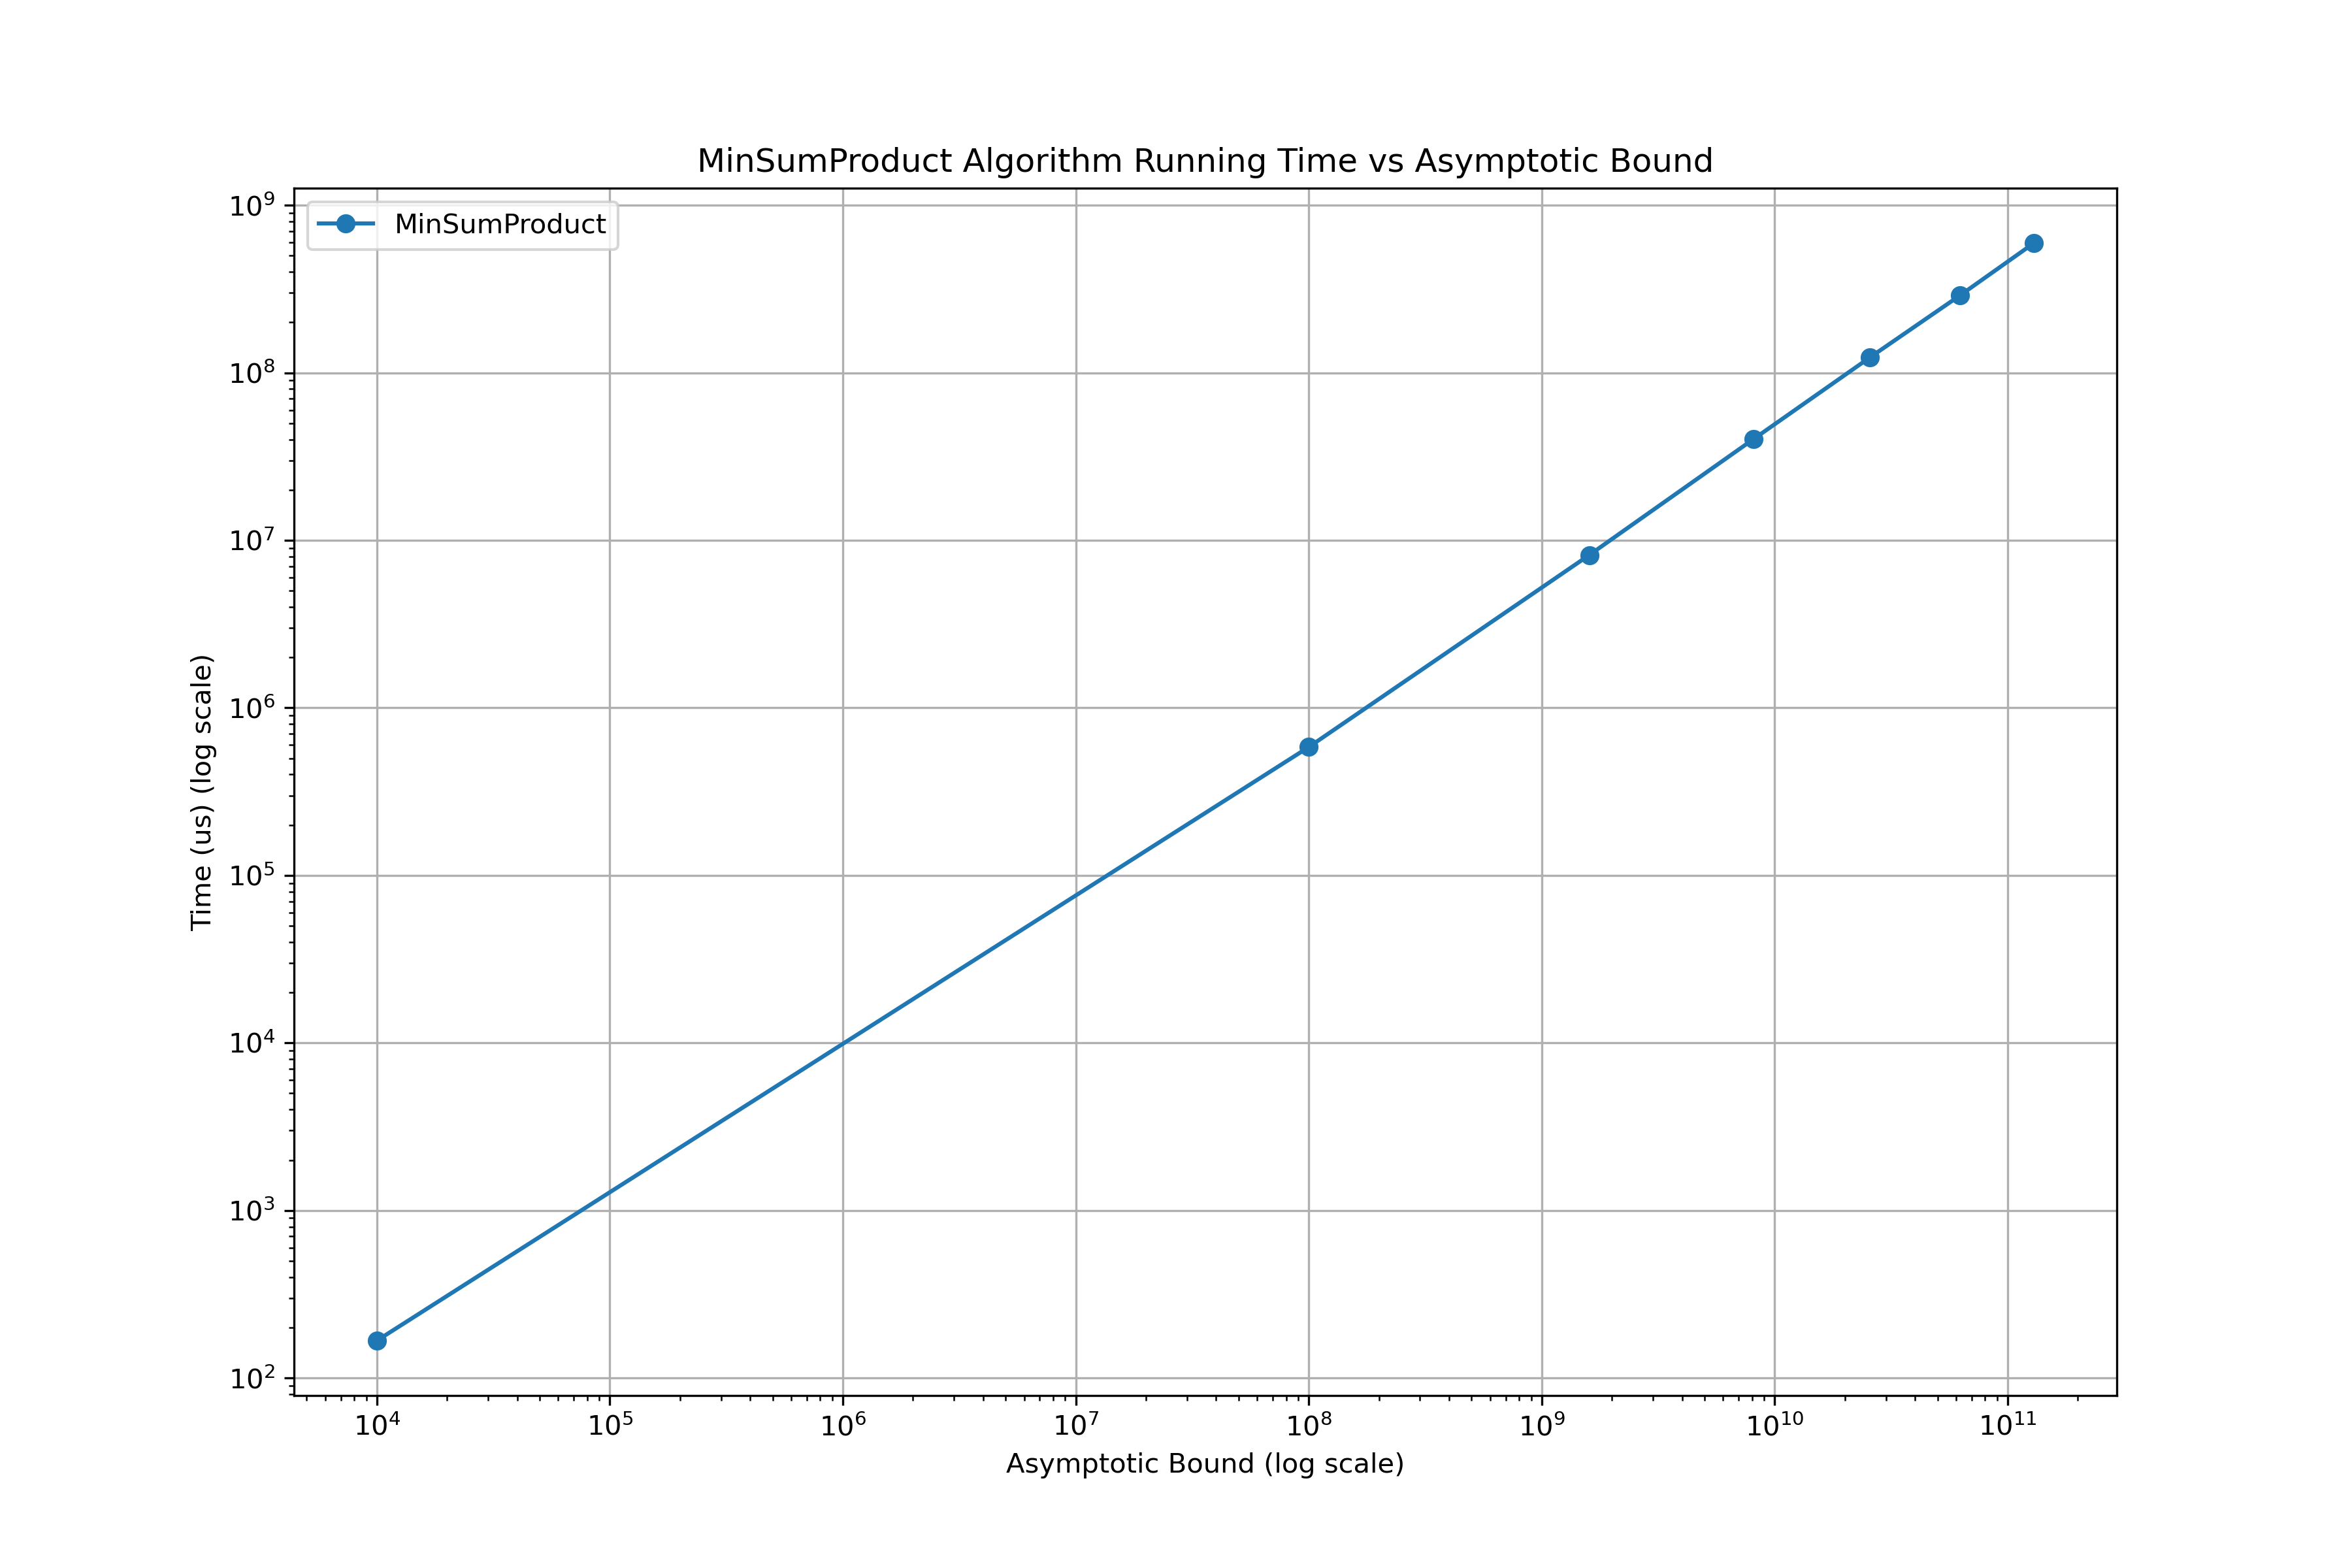
\includegraphics[width=\textwidth]{../results/MinSumProduct_running_time_bound.png}
      \caption{Min-Sum Products}
  \end{subfigure}
  \caption{Different Algorithm runtime - big $O$ bound relationship}
\end{figure}

\subsection{Analysis the result}\

Next, we analyze the meaning and correctness of the above experimental results. Figure 1 is 
drawn only to give an intuitive understanding of the relationship between running time and n. 
According to the definition of big $O$ notation, 
\[
  f(n) = O(g(n)) \iff \exists c, n_0 \text{ s.t. } f(n) \leq c \cdot g(n) \text{ for all } n \geq n_0
\]

In Figure 2, I have labeled the horizontal axis with the theoretical running time $O$ upper bound 
function of each algorithm (denote as $g(n)$). If there is a straight line through the origin, 
when $n>n_0$, this line is always above the experimentally measured running time function $f(n)$; 
Or, viewed on a logarithmic scale, this is equivalent to,
\[
  \log f(n) \leq \log c + \log g(n) \text{ for all } n \geq n_0
\]

i.e. there exist a line with slope $1$ and intercept $\log c$ that is always above the curve $\log f(n)$ in the figure.
It's easy to see that Figure 2 is completely consistent with this theoretical result, and even agrees very well.

Note: I use a logarithmic scale for two reasons: First, the data points are not evenly selected. If we do not use 
a logarithmic scale, most of the points will be crowded in one corner, and a few points will occupy a large part of 
the graph; second, in a logarithmic scale, $c$ parameter become the intercept of the line, which is easier to observe.
(In the non logarithmic scale, $c$ parameter is the slope of the line, which is a little harder to observe.)

\nocite{*}
\bibliographystyle{plain} % or any other style you prefer
\bibliography{references} % use the .bib file
\end{document}